\chapter{M\'ethodologie de recherche}

Dans ce chapitre nous pr\'esentons la d\'emarche exp\'erimentale que
nous avons choisie d{\textquoteright}utiliser pour mener \`a bien cette
recherche, ainsi que les r\'esultats que nous avons obtenus. Nous avons
choisi de nous saisir de diff\'erents outils informatiques,
algorithmiques et de visualisation afin d{\textquoteright}observer les
m\`emes circulant sur Sina Weibo. Nous d\'ebuterons ce chapitre en
discutant des implications d{\textquoteright}une m\'ethodologie
fond\'ee sur l{\textquoteright}analyse et la visualisation de donn\'ees
pour une recherche en sciences sociales. Dans un second temps, nous
brosserons un panorama des m\'ethodes utilis\'ees pour explorer les
donn\'ees issues des r\'eseaux sociaux. Enfin, nous pr\'esenterons
notre d\'emarche ainsi que les r\'esultats de cette \'etude.

\section[Sciences sociales du r\'eseau]{Sciences sociales du r\'eseau}
Pour l{\textquoteright}empiriste, l{\textquoteright}acte essentiel de la
recherche est l{\textquoteright}observation. Structure sch\'ematique
faite de points et de lignes, le r\'eseau n{\textquoteright}offre que
peu de prises pour une approche empirique. Pourtant, ce concept
prot\'eiforme traverse aujourd{\textquoteright}hui les disciplines pour
se retrouver au centre des d\'ebats scientifiques. Coupl\'e \`a
l{\textquoteright}autre grand insaisissable de
l{\textquoteright}\'etude qu{\textquoteright}est
\textit{l{\textquoteright}information, }le mod\`ele du r\'eseau fait la
promesse de nouvelles perspectives en offrant un cadre conceptuel
commun pour les sciences et de nouveaux horizons m\'ethodologiques
gr\^ace aux outils informatiques. L{\textquoteright}interrogation
autour des r\'eseaux se trouve donc plus que jamais au c{\oe}ur du
devenir des sciences.

\subsection[Le r\'eseau comme enjeu pour l{\textquoteright}\'etude]{Le r\'eseau comme enjeu pour l{\textquoteright}\'etude}
Durant la seconde guerre mondiale et jusqu{\textquoteright}\`a la fin
des ann\'ees 1950, les esprits les plus brillants du si\`ecle (G\"odel,
Von Neumann, Einstein..) se c\^otoient \`a
\textit{l{\textquoteright}Institut des Etudes Avanc\'ees} de Princeton
(IAS) aux USA et leurs travaux posent les bases logiques et
technologiques d{\textquoteright}o\`u \'emerge la science informatique
actuelle. Dans le domaine de la philosophie math\'ematique tout
d{\textquoteright}abord, les interrogations amorc\'ees par Russel dans
ses \textit{Principia Mathematica }puis leur critique par G\"odel
dessinent les contours d{\textquoteright}une {\textquotedblleft}machine
r\'ecursive{\textquotedblright}, anc\^etre math\'ematique de la machine
de Turing et de l{\textquoteright}ordinateur de Von Neumann.
Consid\'er\'e comme le p\`ere de l{\textquoteright}ordinateur, Von
Neuman s{\textquoteright}exile d{\textquoteright}Allemagne pour
rejoindre l{\textquoteright}IAS nouvellement fond\'e d\`es 1933 o\`u il
poursuit des recherches dans le domaine de la physique nucl\'eaire. En
1943, Von Neumann int\`egre le \textit{Projet Manhattan} dirig\'e par
Oppenheimer o\`u il est charg\'e de superviser
l{\textquoteright}immense processus de calcul n\'ecessaire \`a la
construction de la bombe qui s{\textquoteright}abattra sur Hiroshima le
6 A\^out 1945. C{\textquoteright}est durant cette p\'eriode que Von
Neumann d\'eveloppe l{\textquoteright}architecture encore utilis\'ee
aujourd{\textquoteright}hui comme base fondamentale du design
\'electronique. Dans ses lectures \`a l{\textquoteright}Universit\'e de
Yale en 1957 parues sous le titre c\'el\`ebre de
\textit{L{\textquoteright}Ordinateur et le Cerveau} \cite{VonNeumann1948}, Von Neumann
identifie les diff\'erentes unit\'es d{\textquoteright}un ordinateur :
unit\'e d{\textquoteright}arithm\'etique logique, unit\'e de
contr\^ole, m\'emoire et entr\'ees/sorties. Les travaux teint\'es
d{\textquoteright}ombre de ce prestigieux math\'ematicien font \'echo
\`a ceux de l{\textquoteright}anglais Turing qui travaille \'egalement
sur la question de l{\textquoteright}intelligence des machines depuis
le d\'ebut de la guerre. Leur correspondance t\'emoigne du respect
mutuel qu{\textquoteright}entretiennent alors les deux savants, ainsi
que leurs nombreux questionnements sur la possibilit\'e
d{\textquoteright}une machine intelligente \cite{Istrail2013}.
Au c{\oe}ur de leurs discussions se trouve la qu\^ete
d{\textquoteright}un mod\`ele universel capable
d{\textquoteright}expliquer le fonctionnement de
l{\textquoteright}activit\'e cognitive. 

Norbert Wiener, un autre prodige des math\'ematiques prend \'egalement
part \`a cette recherche. Sa th\'eorie qu{\textquoteright}il nomme
\textit{cybern\'etique }place la notion d{\textquoteright}information
au c{\oe}ur de la r\'eflexion sur le fonctionnement des syst\`emes :
\textit{{\textquotedblleft}Information is information, not matter or
energy{\textquotedblright}} \cite{VonNeumann1948}, p. 155). Utilisant les concepts de
bruit, de messages et de \textit{feedbacks}, il jongle entre
math\'ematiques appliqu\'ees et sciences cognitives pour comprendre les
ph\'enom\`enes de transmission de signaux complexes. Dans une lettre du
29 Novembre 1946, Von Neumann \'ecrit \`a Wiener que
l{\textquoteright}\'etude du cerveau {\textquotedblleft}\textit{the
most complicated object under the sun, litterally}{\textquotedblright}
n\'ecessite de poursuivre une r\'eflexion transverse \`a de multiples
disciplines scientifiques \cite{Masani1990}. Depuis le d\'ebut de cette
m\^eme ann\'ee 1946, les {\textquotedblleft}conf\'erences
cybern\'etiques{\textquotedblleft} aussi connues sous le nom de
{\textquotedblleft}conf\'erences Macy{\textquotedblright} ont
d\'ebut\'e \`a New York dans le but de d\'efinir
\textit{{\textquotedblleft}une science g\'en\'eral de
l{\textquoteright}esprit humain{\textquotedblright}}\footnote{
Foundation for Cybernetics, The Macy Conferences
\url{http://www.asc-cybernetics.org/foundations/history/MacySummary.htm}
consult\'e le 10 Mars 2014 \`a 16h16 GMT+1}. Regroupant physiciens,
cogniticiens, biologistes, anthropologues et linguistes, ces
conf\'erences sont l{\textquoteright}objet de nombreuses publications
dont \textit{The Human Use of Human Beings} \cite{Wiener1954} qui propose
d{\textquoteright}\'etudier la soci\'et\'e en consid\'erant les
communications entre hommes et machines. Le travail men\'e lors de ces
conf\'erences est souvent consid\'er\'e comme la pierre fondatrice du
champ des \'etudes sur la communication \cite{Breton1998, Winkin1981}.
Quelques ann\'ees plus tard, McLuhan et son id\'ee controvers\'ee de
\textit{village global} \cite{MacLuhan1962} am\`enent un large auditoire autour des
{\oe}uvres de Wiener et l{\textquoteright}\'etude des modes de
communication. Progressivement se constitue un champ
\'epist\'emologique pour l{\textquoteright}\'etude de
l{\textquoteright}information dont la d\'efinition reste encore
aujourd{\textquoteright}hui un enjeu important \cite{Wolton1997}. En
France, les Sciences de l{\textquoteright}Information et de la
Communication se sont principalement structur\'ees autour de la
critique des m\'edias \cite{Mattelart1979, Debray1979} dans une
tradition europ\'eenne d\'ej\`a bien install\'ee \cite{Adorno1944}. Aux Etats-Unis, les \textit{cultural studies }\cite{Hall1970}
s{\textquoteright}interrogent davantage sur
l{\textquoteright}\'economie politique des symboles et trouvent leur
lettres de noblesse dans les \textit{media studies,
}aujourd{\textquoteright}hui devenue une discipline universitaire
reconnue en Angleterre et aux USA. Toutefois,
l{\textquoteright}\'emergence d{\textquoteright}un
\textit{{\textquotedblleft}paradigme
communicationnel{\textquotedblright} }\cite{Bougnoux1998} n\'ecessite un
dialogue pas toujours \'evident entre les diff\'erentes disciplines
constitu\'ees autour de l{\textquoteright}\'etude des pratiques de
l{\textquoteright}information et de la communication : sociologie des
m\'edias, \'etudes des syst\`emes d{\textquoteright}information,
informatique, sciences de l{\textquoteright}information et de la
communication, etc. 

Alors que le programme fix\'e par la cybern\'etique a pour ambition
d{\textquoteright}explorer les structures, possibilit\'es et
contraintes des syst\`emes communicants, l{\textquoteright}image
ferm\'ee et cyclique du syst\`eme devient rapidement trop \'etriqu\'ee
pour une r\'eflexion sur les relations en pleine expansion. Deleuze et
Guattari proposent dans l{\textquoteright}introduction de leur livre
\textit{Milles Plateaux} \cite{Deleuze1972} de s{\textquoteright}\'eloigner de
l{\textquotesingle}arborescence classique du syst\`eme auto-suffisant
pour envisager les liens entre sujets et objets sous la forme ouverte
et combinatoire du \textit{rhizome. }Le rhizome se d\'efinit par son
caract\`ere non-fini et fait de l{\textquoteright}\'etude des
causalit\'es un ph\'enom\`ene contextuel aux sp\'ecificit\'es pas
forc\'ement reproductibles. Imperm\'eable \`a la cat\'egorisation et
aux classifications ordonn\'es, l{\textquoteright}objet
d{\textquoteright}\'etude in-form\'e devient \textit{open-ended},
moment donn\'e \`a voir et \'etat unique d{\textquoteright}un ensemble
plus vaste. La v\'erit\'e ou la validit\'e n{\textquoteright}est donc
plus \`a d\'ecouvrir dans l{\textquoteright}analyse, mais plut\^ot dans
l{\textquoteright}articulation des contingences entre objets et
environnements dont se saisit le champ \'emergent des \'etudes sur la
complexit\'e \cite{Morin2005}. Dans le m\^eme temps, les progr\`es de
l{\textquoteright}intelligence artificielle et de la robotique viennent
\'egalement questionner notre d\'efinition du vivant face \`a ces
nouveaux \^etres \cite{Hofstadter1999}. Le mod\`ele du \textit{r\'eseau
}vient \`a son tour in-former la pens\'ee scientifique comme un nouvel
\textit{episteme }foucaldien offrant une grille de lecture des faits
sociaux renouvel\'ee \cite{Castells1989, Latour1996}.
Aujourd{\textquoteright}hui, la structuration d{\textquoteright}un
champ de recherche coh\'erent et multi-disciplinaire autour de
l{\textquoteright}\'etude des r\'eseaux reste un enjeu important pour
le monde de la recherche \cite{Brandes2013}. Cette consid\'eration
pour la complexit\'e des ph\'enom\`enes permet en effet
d{\textquoteright}imaginer une approche scientifique qui att\'enuerait
les liens entre des disciplines dont le dialogue parfois difficile est
n\'eanmoins n\'ecessaire, afin de mener vers une r\'econciliation des
sciences humaines, des sciences naturelles et des sciences du vivant
o\`u cohabiteraient
\textit{{\textquotedblleft}l{\textquoteright}\'etude des organismes,
des organes et des organisations{\textquotedblright} }\cite{Morin2005}

\subsection[Code, donn\'ees et les nouveaux outils de l{\textquoteright}\'ecriture scientifique ]{3.1.2. Code, donn\'ees et les nouveaux outils de l{\textquoteright}\'ecriture scientifique }
Les objets ouverts et mal d\'efinis du r\'eseau posent n\'eanmoins la
question d{\textquoteright}une continuit\'e avec le projet
aristot\'elicien d{\textquoteright}une compr\'ehension du monde par le
savoir analytique. La consid\'eration d{\textquoteright}un objet comme
moment du r\'eseau rend caduque l{\textquoteright}id\'ee de sa
d\'efinition \textit{a priori, }en dehors des relations
qu{\textquoteright}il entretient avec son environnement. A
l{\textquoteright}inverse, une d\'efinition des objets entre origine,
fonction et destination ne devrait pas \'eluder non plus la r\'eflexion
ontologique autour de son \textit{\^etre}. Le philosophe am\'ericain
William James propose une m\'ethode qu{\textquoteright}il nomme
\textit{empirisme radical }o\`u l{\textquoteright}existence des objets
doit \^etre consid\'er\'ee par le prisme de
l{\textquoteright}exp\'erience \cite{James1912}\textit{.
}L{\textquoteright}exp\'erience, m\^eme scientifique, existe dans un
contexte, un lieu, un temps, un moment, une succession
d{\textquoteright}\'etapes, et c{\textquoteright}est cet ensemble qui
nous permet de percevoir les ph\'enom\`enes \'etudi\'es. Si
l{\textquoteright}acte essentiel de l{\textquoteright}empiriste et du
philosophe est l{\textquoteright}observation, alors elle doit \^etre
radicale dans son honn\^etet\'e et accepter
l{\textquoteright}exp\'erience dans son unicit\'e dont de nombreux
facteurs sont non-reproductibles. Cette question de
l{\textquoteright}exp\'erience et de sa reproductibilit\'e est depuis
toujours au c{\oe}ur du d\'ebat sur les sciences et se pose comme un
des ressorts fondamentaux du savoir scientifique. Les sciences dites
{\textquotedblleft}dures{\textquotedblright} comme la physique, la
biologie, l{\textquoteright}informatique ou m\^eme la g\'eologie
valident leurs hypoth\`eses gr\^ace \`a l{\textquoteright}usage
extensif d{\textquoteright}appareillages multiples devenus une cl\'e de
la reproductibilit\'e des exp\'eriences. Du simple microscope \`a
l{\textquoteright}acc\'el\'erateur du CERN, la m\'ethodologie
d{\textquoteright}observation est pour ces disciplines souvent
indissociable de la technologie. Le travail de la recherche et de la
preuve s{\textquoteright}articule ici autour des trois p\^oles de la
th\'eorie, de l{\textquoteright}exp\'erience et de la m\'ethode
conditionn\'ee \`a la technique. 


\begin{figure}
    \centering
    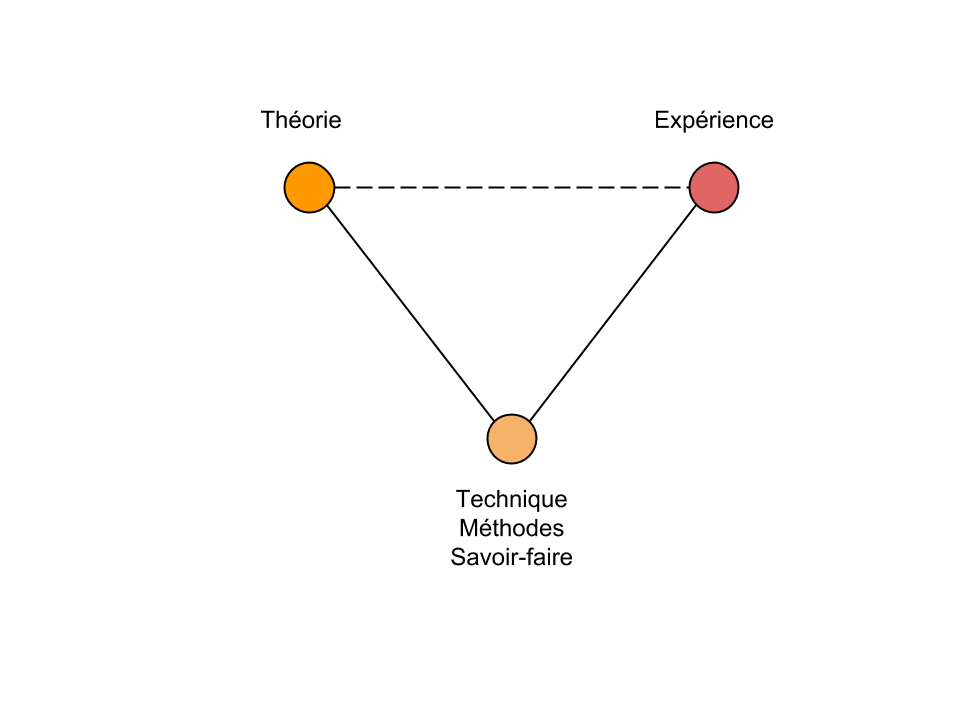
\includegraphics[width=5.0559in,height=3.7894in]{figures/chap3/chapitre3-img1.png}
    \caption[Triptyque des pratiques scientifiques]{Triptyque des pratiques scientifiques}
\end{figure}


En sciences humaines n\'eanmoins, la tension entre la th\'eorie (les
concepts), l{\textquoteright}exp\'erience (le terrain) et la
m\'ethodologie s{\textquoteright}articule plus rarement autour
d{\textquoteright}outillages \'elabor\'es. Les \ r\'eflexions sur la
m\'ethodologie en sciences sociales portent plus largement sur des
argumentations conceptuelles o\`u le langage lui-m\^eme est
consid\'er\'e comme l{\textquoteright}outil premier ou encore de
nombreuses r\'eflexions \'ethiques sur l{\textquoteright}impact des
pratiques d{\textquoteright}observation dans le cadre de
l{\textquoteright}anthropologie notamment. En France,
l{\textquoteright}int\'er\^et constant port\'e \`a
l{\textquoteright}utilisation des diff\'erentes formes de technologie
en sciences humaines s{\textquoteright}est souvent constitu\'e autour
de la critique de m\'ethodologies quantitatives tr\`es r\'epandues
outre atlantique - la statistique en sociologie,
l{\textquoteright}\'etude comportementaliste en psychologie ou le film
ethnographique \cite{Becker1974}. Comme le note justement Latour, la
qu\^ete de l\'egitimit\'e des Sciences Sociales s{\textquoteright}est
souvent traduit par une capacit\'e \`a se procurer et traiter des
donn\'ees : \textit{{\textquotedblleft}Sociology has been obsessed by
the goal of becoming a quantitative science.{\textquotedblright}}
\cite{Latour2010}. Pourtant, il serait illusoire de corr\'eler la
quantit\'e de donn\'ees \`a une quelconque objectivit\'e de la
d\'emarche scientifique, tant les d\'emarches et outils n\'ecessaires
pour la collecte sont en soi autant de biais importants. La question de
la r\'eussite des \'etudes utilisant les Big Data semblent davantage
corr\'el\'ee \`a la capacit\'e d{\textquoteright}une approche
m\'ethodologique forg\'ee dans un \'echange interdisciplinaire et des
pratiques renouvel\'ees de l{\textquoteright}\'ecriture. La
complexit\'e des questions abord\'ees lors du traitement des donn\'ees,
non seulement technologique mais aussi dans les interrogations sur la
l\'egitimit\'e de leur existence, leur utilisation et leur provenance
\cite{Boyd2011} rendent n\'ecessaire la discussion entre de
multiples connaissances. Aujourd{\textquoteright}hui,
l{\textquoteright}utilisation de l{\textquoteright}ordinateur
conditionne l{\textquoteright}\'ecriture scientifique de
l{\textquoteright}\'etude de terrain, la prise de notes, la r\'edaction
ou la publication et se pr\'esente ainsi comme un imp\'eratif
m\'ethodologique pour la r\'eflexion et le travail en sciences humaines
et sociales \cite{Wieviorka2013}. L{\textquoteright}appareillage projet\'e
au centre de la pratique quotidienne du chercheur vient modifier le
travail de r\'eflexion sur les ph\'enom\`enes \'etudi\'es et
s{\textquoteright}accompagne de multiples contraintes. La prise en main
de ce nouvel \textit{{\textquotedblleft}instrument
intellectuel{\textquotedblright} }\cite{Guichard2014} passe par une lente
alphab\'etisation aux langages des machines. L{\textquoteright}angoisse
latente du {\textquotedblleft}bug{\textquotedblright}
n{\textquoteright}est pas apais\'ee par les rares techniciens
pr\'esents dans les centres de recherche en sciences humaines, souvent
d\'ej\`a d\'epass\'es par la diversit\'e des demandes technologiques.
L{\textquoteright}\'ecriture, savoir-faire indispensable de la
recherche, poss\`ede une nouvelle mat\'erialit\'e dans les disques durs
produisant une d\'ependance accrue aux r\'eseaux
d{\textquoteright}ordinateurs. Cette empreinte
{\textquotedblleft}digitale{\textquotedblright} laiss\'ee par les
calculateurs sur les pratiques scientifiques n{\textquoteright}est ni
anodine ni r\'evolutionnaire et s{\textquoteright}inscrit dans la
longue tradition des cultures de l{\textquoteright}\'ecrit qui d\'ej\`a
bien avant les moines copistes \textit{{\textquotedblleft}combinent les
gestes de la main et les op\'erations de la
pens\'ee.{\textquotedblright}} \cite{Jacob2011} 

Tim Berners-Lee, consid\'er\'e comme l{\textquoteright}inventeur du
World Wide Web et du Web S\'emantique d\'efinit la constitution
d{\textquoteright}un r\'eseau mondial des savoirs comme un projet
d{\textquoteright}\textit{{\textquotedblleft}ing\'enierie
philosophique{\textquotedblright} }\cite{Halpin2014}.
Mi-philosophe mi-ing\'enieur, le chercheur contribuant \`a ce r\'eseau
de savoir doit donc \^etre en capacit\'e de conna\^itre les protocoles
et les langages pour y acc\'eder et s{\textquoteright}y mouvoir
ais\'ement. La m\'ethode scientifique s{\textquoteright}\'ecrit
notamment avec de nouvelles formulations (fonctions, algorithmes,
code...). Les donn\'ees g\'en\'er\'ees par les usages
d{\textquoteright}un nombre croissant de machines communicantes et
productrices d{\textquoteright}information, souvent d\'esign\'ees par
le concept {\guillemotleft}~valise~{\guillemotright} de Big Data \cite{Lohr2012} offrent des possibilit\'es nouvelles pour
l{\textquoteright}\'etude en sciences sociales.
L{\textquoteright}analyse de ces vastes jeux de donn\'ees
s{\textquoteright}accompagne \'egalement de nouveaux imp\'eratifs et
questionnements sur l{\textquoteright}observation des ph\'enom\`enes
humains qu{\textquoteright}ils repr\'esentent. \`A la fois barri\`ere
et opportunit\'e, une difficult\'e majeure r\'eside dans le
discernement n\'ecessaire entre praxis des outils informatiques,
fascination pour ces outils et r\'eflexions pertinentes sur la
qualit\'e des m\'ethodes employ\'ees. Le traitement quantitatif par
ordinateur permet d{\textquoteright}extraire de nombreuses
connaissances utiles de jeux de donn\'ees parfois tr\`es importants
mais n{\textquoteright}assure pas pour autant la qualit\'e des
r\'esultats. Une bonne compr\'ehension de la provenance et des
m\'ethodes de collection des donn\'ees est n\'ecessaire afin
d{\textquoteright}identifier des algorithmes de traitements
int\'eressants, adapt\'es et efficaces parmi ceux disponibles
\cite{Rajaraman2011}. Les m\'ethodologies
d{\textquoteright}exploration et de recherche utilisant le
{\textquotedblleft}Big Data{\textquotedblright} comme source
n\'ecessite la mise en {\oe}uvre d{\textquoteright}une ing\'enierie
complexe soutenu par une connaissance des technologies n\'ecessaires
\`a l{\textquoteright}analyse de donn\'ees.
L{\textquoteright}algorithmique, la statistique,
l{\textquoteright}informatique mais \'egalement la cartographie et le
design graphique doivent se conjuguer pour permettre de produire des
r\'esultats \`a la fois int\'eressants et fiables. Ce travail
d{\textquoteright}hypoth\`eses et de v\'erifications pour
l{\textquoteright}analyse de donn\'ees doit r\'eunir de nombreuses
comp\'etences. La d\'efinition de la probl\'ematique la plus adapt\'ee
n\'ecessite une connaissance aig\"ue du terrain et des outils et
algorithmes qui seront articul\'es au sein d{\textquoteright}un
syst\`eme ing\'enierique parfois tr\`es complexe. Le design et la
lecture d{\textquoteright}algorithme pour le
\textit{{\textquotedblleft}data mining{\textquotedblleft}} sont donc
les cl\'es pour le travail du chercheur confront\'e aux donn\'ees.
N\'eanmoins, ces algorithmes ne devraient \^etre que la traduction de
questions formul\'ees gr\^ace \`a une connaissance aig\"ue des
probl\'ematiques du contexte et des objets \'etudi\'es - notamment pour
identifier les donn\'ees manquantes. La {\textquotedblleft}science des
donn\'ees{\textquotedblright} promet donc d{\textquoteright}apporter un
v\'eritable renouveau des m\'ethodes et des r\'esultats scientifiques,
au prix d{\textquoteright}un travail soutenu pour faire face \`a ces
changements d{\textquoteright}habitudes et de langages. Les
applications statistiques du {\textquotedblleft}big
data{\textquotedblright} permettent aujourd{\textquoteright}hui une
fiabilit\'e accrue des pr\'edictions par l{\textquoteright}augmentation
du volume des corpus trait\'es \cite{Breiman2001}. Le domaine de
l{\textquoteright}intelligence artificielle (AI) a grandement
b\'en\'efici\'e de l{\textquoteright}accroissement de la capacit\'e de
traitement des donn\'ees notamment pour la pr\'ediction gr\^ace au
techniques dites de \textit{machine learning}. N\'eanmoins Peter
Norvig, directeur de recherche chez Google, reconnait lui-m\^eme :
{\textquotedblleft}\textit{We could draw this curve: as we gain more
data, how much better does our system get? And the answer is,
it{\textquoteright}s still improving---but we are getting to the point
where we get less benefit than we did in the past.{\textquotedblright}
}\cite{Somers2013}. Comme le note Douglas Hofstadter, un des pairs de
l{\textquoteright}Intelligence Artificielle \`a propos du
super-ordinateur qui venait de battre Kasparov aux \'echecs :
\textit{{\textquotedblleft}Okay, Deep Blue plays very good chess---so
what? Does that tell you something about how we play chess? No. Does it
tell you about how Kasparov envisions, understands a
chessboard?{\textquotedblright} }\cite{Somers2013}. 

En effet, ces pratiques m\'ethodologiques doivent r\'eussir \`a
s{\textquoteright}inscrire dans la continuit\'e de
l{\textquoteright}historicit\'e et des exigences des disciplines. La
portabilit\'e des m\'ethodes et la disponibilit\'e des donn\'ees sont
encore des questions centrales et non-r\'esolues. En sciences sociales
notamment, les services de r\'eseaux sociaux en ligne offrent de tr\`es
large corpus dont l{\textquoteright}utilisation est r\'egie par les
exigences commerciales des soci\'et\'es priv\'ees qui les d\'etiennent.
L{\textquoteright}analyse des donn\'ees issues de service de r\'eseaux
sociaux en ligne est pourtant un champ d{\textquoteright}\'etudes en
rapide expansion \cite{Nettleton2013}. Pourtant, le d\'ebat sur la
validit\'e des \'eclairages apport\'es par l{\textquoteright}analyse
des donn\'ees issues des services de r\'eseaux reste encore largement
ouvert et nous entendons dans ce travail de recherche y contribuer. 

\subsection[Visualisation et espace perceptif pour l{\textquoteright}information]{3.1.3 Visualisation et espace perceptif pour l{\textquoteright}information}
Face \`a de larges volumes de donn\'ees, un des grands enjeux est
d{\textquoteright}en restituer une forme intelligible afin de
d{\textquoteright}identifier des tendances ou des motifs particuliers.
La visualisation permet de produire une lecture particuli\`ere de
parties int\'eressantes et intelligibles d{\textquoteright}un jeu de
donn\'ees \cite{Cairo2013}. D\'efinie comme \textit{{\guillemotleft}~a
process that transforms data, information, and knowledge into a form
that relies on the human visual system to perceive its embedded
information.{\textquotedblright}} \cite{Graffieti2010}, la
visualisation introduit la question du design visuel au c{\oe}ur de la
probl\'ematique d{\textquoteright}analyse \cite{Wesolowsky1992}.
La visualisation correspond \`a une s\'erie d{\textquoteright}actions
qui r\'esulte dans la production de marqueurs visuels (points, ligne,
aires, surface, volume) avec comme \'etapes la d\'efinition de leurs
propri\'et\'es r\'etiniennes (couleur, taille, texture, etc.) et leur
positionnement dans l{\textquoteright}espace visuel \cite{Card Mackinlay}
 \`a d\'efinir les bases d{\textquoteright}une grammaire de la
visualisation en commen\c{c}ant par en identifier les formes
syntaxiques : 

\begin{enumerate}
\item les objets graphiques montr\'es (ex. point, fl\`eche, pictogramme,
etc.), 
\item l{\textquoteright}espace graphique donnant sens \`a
l{\textquoteright}organisation des objets (ex. syst\`emes de
coordonnn\'ees g\'eographiques, timeline, etc.),
\item les propri\'et\'es graphiques des objets (couleurs, tailles,
etc.),
\item l{\textquoteright}organisation des objets en diff\'erentes
cat\'egories~(ex. cadre, liens, l\'egendes, etc.). 
\end{enumerate}
Ces choix forment une t\^ache importante dont l{\textquoteright}enjeu
n{\textquoteright}est pas seulement visuel, mais se joue \'egalement
dans le champ de la repr\'esentation o\`u les objets sont donn\'es \`a
voir et par l\`a-m\^eme donn\'es \`a comprendre. Les travaux sur
l{\textquoteright}apparition de la perspective dans la Renaissance
italienne ont montr\'e comment l{\textquoteright}espace de la
repr\'esentation visuelle fait \'echo aux changements soci\'etaux
profonds de l{\textquoteright}\'epoque \cite{Raynaud2005}. Au-del\`a
d{\textquoteright}une simple technique picturale, les {\oe}uvres des
peintres du Quattrecento t\'emoignent de changements profonds dans la
perception : l{\textquoteright}espace perceptif se structure
d\'esormais autour du sujet et \ de son {\textquotedblleft}point de
vue{\textquotedblright} qui construit l{\textquoteright}ensemble de la
repr\'esentation \cite{Damisch1999}. Empreinte de rationalit\'e, la
perspective construit comme au th\'e\^atre un espace de
repr\'esentation centr\'e autour du spectateur. En 1639, le
math\'ematicien Desargues mod\'elise les notions intuitives de
perspective et d{\textquotesingle}horizon gr\^ace \`a la g\'eom\'etrie
projective qui permet d{\textquoteright}\'etudier les propri\'et\'es
inchang\'ees des figures lors de leur projection. Cette g\'eom\'etrie
d{\textquoteright}un genre nouveau se structure autour du \textit{plan
projectif}, \'el\'ement topologique qui
\textit{{\textquotedblleft}rassemble en une seule surface
l{\textquoteright}imagination de tous les points de vue
possible{\textquotedblright} }\cite{Petit1996}. En construisant un plan
g\'eom\'etrique fond\'e sur le point de vue, de nouveaux \^etres
g\'eom\'etriques aux propri\'et\'es \'etranges voient le jour, dont
l{\textquoteright}existence logique force notre repr\'esentation
classique : la bande de M\"obius ne poss\`ede qu{\textquoteright}une
seule face et il est impossible de distinguer
l{\textquoteright}int\'erieur de l{\textquoteright}ext\'erieur
d{\textquoteright}une bouteille de Klein. Dans ces surfaces dites
\textit{unilat\`eres}, le local est travers\'e en tout point par un
tout global. Nous ne pouvons pas traverser puisque nous somme toujours
sur la m\^eme face. Ni bord, ni ext\'erieur, ni int\'erieur, le plan
projectif apporte des \'el\'ements de r\'eponses conceptuelles aux
limites des la repr\'esentation dans l{\textquoteright}espace. 

Dans le contexte de syst\`emes et de r\'eseaux complexes, la
visualisation de donn\'ees structure l{\textquoteright}espace perceptif
afin de construire une sc\`ene \`a \textit{n }dimensions dont
l{\textquoteright}enjeu est la recherche d{\textquoteright}un
{\textquotedblleft}point de vue{\textquotedblright} pour
l{\textquoteright}\'etude\textit{. }Alors que la perspective prend pour
parti de mat\'erialiser le sujet au centre de la repr\'esentation par
des points de fuite, la visualisation de donn\'ees cherche elle \`a
utiliser les objets comme dimensions du champ de la repr\'esentation,
en structurant souvent l{\textquoteright}espace autour de quantit\'es.
N\'eanmoins, la place du spectateur / utilisateur dans la visualisation
reste un des enjeux majeurs encore \`a explorer. En \'elaborant sa
{\textquotedblleft}m\'ethode graphique{\textquotedblright} , J.E. Marey
\cite{Marey1885} utilise la photographie pour cr\'eer un nouvel espace de
repr\'esentation du mouvement et observer des ph\'enom\`enes
jusqu{\textquoteright}ici invisibles. Si la temporalit\'e de
l{\textquoteright}\'ecrit ou de la voix est avant lin\'eaire,
l{\textquoteright}espace visuel permet de manier le r\'eel pour le
d\'ecomposer en actes logiques. Charcot cherche dans les images de
l{\textquoteright}hyst\'erie des t\'emoignages de la folie et proc\`ede
\`a la mise en sc\`ene de ses patients dans ce nouvel espace de
repr\'esentation ouvert par la photographie \cite{Didi-Huberman2012}.

La visualisation scientifique se pr\'evaut donc d{\textquoteright}une
existence avant tout pratique dont le premier objectif serait de
\textit{{\guillemotleft}~to effectively convey
information~{\guillemotright}} \cite{Kelleher2011}. Son
caract\`ere syncr\'etique et sa capacit\'e \`a r\'esumer une large
masse d{\textquoteright}information rapidement en font un des plus
importants \'el\'ements de la publication en science notamment pour sa
diffusion et la facilitation d{\textquoteright}acc\`es \`a une
connaissance \cite{Ware2004}. Dans sa s\'emiologie graphique, Bertin
\cite{Bertin1977} distingue deux usages majeurs des graphiques de visualisation :
1) un moyen de communiquer des informations (dans le cas o\`u
l{\textquoteright}information a d\'ej\`a \'et\'e comprise) 2) un moyen
visuel de r\'esoudre des probl\`emes logiques (quand le graphique est
utilis\'e comme support de lecture et de manipulation
d{\textquoteright}informations). Ces deux caract\'eristiques peuvent
coexister dans certaines pi\`eces mais la transition entre les deux
n\'ecessite souvent un travail important de restructuration visuelle.
Dans le traitement et la la visualisation des donn\'ees
\textit{l{\textquoteright}interface }joue un r\^ole primordial. On peut
d\'esormais agir sur la 2\`eme cat\'egorie de Bertin pour mieux
explorer le sens \cite{Weissberg2007}. Manovich montre comment
l{\textquoteright}interface d\'efinie comme
\textit{{\textquotedblleft}the ways to represent
({\textquoteleft}format{\textquoteright}) and control the
signal.}{\textquotedblright} \cite{Manovich2013}. Ce formatage nouveau de
l{\textquoteright}information induit des changements dans la pratique
de la lecture qui, toujours selon Manovich,
s{\textquoteright}apparenterait davantage \`a de la reconnaissance de
\textit{pattern}, symbolis\'e par l{\textquoteright}usage de
l{\textquoteright}ic\^one et du menu en design
d{\textquoteright}interface. Ainsi si l{\textquoteright}interface
contraint la lecture, la prise en compte des formes narratives (les
\textit{patterns} de Manovich) prend une grande importance quand il
s{\textquoteright}agit de concevoir une visualisation
d{\textquoteright}information. L{\textquoteright}usage des signes
graphiques doit se faire avec une connaissance des usages de
l{\textquoteright}interface, afin de recr\'eer la coop\'eration
textuelle des r\^oles de lecteur et de designer/auteur n\'ecessaire
pour la production un sens \cite{Eco1985}. La \textit{citizen science} ou
encore \textit{night science} a fait de l{\textquoteright}interface un
paradigme en utilisant la visualisation pour amener un grand nombre de
collaborateurs \`a explorer et analyser de vastes jeux de donn\'ees en
effectuant des t\^aches simples \cite{Silvertown2009}. Le projet
\textit{Eyewire} permet \`a des internautes de contribuer \`a la
classification d{\textquoteright}images du cerveau humain en vue de la
r\'ealisation d{\textquoteright}un mod\`ele 3D \cite{Seung2012}. Utilisant
des scans de tranches de 1mm r\'ealis\'es par
l{\textquoteright}institut Max Planck, la mod\'elisation 3D
d{\textquoteright}un cerveau complet promet une belle contribution pour
la d\'ecouverte des fonctionnements cognitifs. N\'eanmoins, la t\^ache
est colossale et n\'ecessiterait plusieurs ann\'ees pour une \'equipe
classique de scientifiques. \textit{Eyewire} propose donc une interface
web o\`u un simple jeu de coloriage permet d{\textquoteright}identifier
les neurones et de contribuer ainsi au dessin du mod\`ele 3D.

Cartes, code ou graphiques, les nouveaux outils num\'eriques participent
donc \`a structurer de nouvelles pratiques de l{\textquoteright}espace
gr\^ace \`a la construction de nouvelles repr\'esentations. 

\section[M\'ethodes et outils d{\textquoteright}analyse des r\'eseaux sociaux]{M\'ethodes et outils d{\textquoteright}analyse des r\'eseaux sociaux}

Nous allons maintenant regarder comment l{\textquoteright}analyse des
donn\'ees des services de r\'eseaux sociaux en ligne (SNA) peut
permettre d{\textquotesingle}interroger les pratiques des technologies
num\'eriques pour mieux en comprendre les tenants.

\subsection[Anatomie d{\textquoteright}un r\'eseau social]{ Anatomie d{\textquoteright}un r\'eseau social}
La repr\'esentation des relations sociales sous forme de graphe trouve
son origine dans les travaux des psychologues allemands de la
\textit{gestalt }durant les ann\'ees 1920-1930 \cite{Scott1988}\textit{.
}S{\textquoteright}inspirant des \'etudes sur le cerveau, le
psychologue J. L. Moreno s{\textquoteright}applique notamment \`a
comprendre les principes organisationnels holistiques des groupes
humains et fonde la sociom\'etrie avec comme objectif la qualification
et la quantification des relations sociales \cite{Moreno1938}.
Moreno cherche \`a identifier et isoler des leaders de groupes sociaux
d\'efinis en \'etudiant l{\textquoteright}asym\'etrie ou la
r\'eciprocit\'e de leurs choix et fr\'equentations amicales. Cherchant
des moyens de repr\'esenter les tendances \`a
l{\textquoteright}auto-organisation qu{\textquoteright}il observe, il
cartographie les relations directes et indirectes entre personnes sous
forme de \textit{sociogrammes}. Les anthropologues
s{\textquoteright}emparent rapidement de ce type
d{\textquoteright}outils pour comprendre les formes tribales (Lundberg,
1936) et l{\textquoteright}\'emergence progressive de la topologie
comme domaine important des math\'ematiques vient d\'efinir de nouveaux
types de relations entre objets disparates, avec notamment la th\'eorie
des graphes qui donne \`a l{\textquoteright}\'etude des r\'eseaux ses
mod\`eles logiques \cite{Harary1977}. Milgram \cite{Milgram1969} voit les relations
humaines comme autant de petits mondes (\textit{small-worlds)}
connect\'es entre eux. Granovetter s{\textquoteright}int\'eresse \`a
l{\textquoteright}importance des relations t\'enues et lointaines
(\textit{weak ties}) dans l{\textquoteright}acquisition
d{\textquoteright}informations importantes \cite{Granovetter1974}.
L{\textquoteright}influence de la th\'eorie des graphes am\`ene
notamment les sociologues \`a exp\'erimenter de nouveaux mod\`eles
venus de la physique ou de la biologie, en proposant de nouvelles
pratiques comme celle de la simulation sociale \cite{Epstein1996}.



La mat\'erialit\'e de l{\textquoteright}image du \textit{graphe}
structure la repr\'esentation du r\'eseau social. Dans la litt\'erature
concernant les r\'eseaux, les notions de graphe et de r\'eseau sont
interd\'ependantes et la th\'eorie des graphes sert notamment de
syst\`emes de notation pour la mise en \'equation des r\'eseaux
\cite{Nettleton2013}. Si cette structure point-ligne semble toutefois
rev\^etir une limite de taille pour la description de ph\'enom\`enes
humains (comment en effet r\'eduire les relations humaines \`a une
simple ligne?), elle semble n\'eanmoins aujourd{\textquoteright}hui
encore difficile \`a d\'epasser.

\begin{figure}
    \centering
    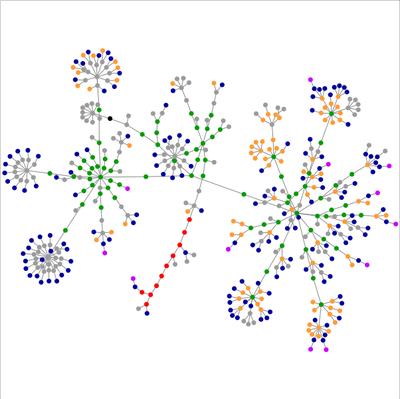
\includegraphics[width=4.178in,height=4.1449in]{figures/chap3/chapitre3-img2.png}
    \caption{Représentation d'un r\'eseau sous forme de graphes.}
\end{figure}


Un r\'eseau consid\'er\'e comme graphe, not\'e \textit{G}, se compose
d{\textquoteright}un ensemble de nodes ou vertices (les points) et de
liens ou edges (les traits). On repr\'esente ainsi un graphe sous la
notation \textit{G(V,E)} o\`u \textit{V }est l{\textquoteright}ensemble
des nodes du r\'eseau et \textit{E} l{\textquoteright}ensemble des
liens\textit{ }d\'ecrivant leurs relations. \textit{E }d\'ecrit les
relations entre les nodes qui peuvent \^etre directionnelles (paires de
vertices ordonn\'ees) dans le cas d{\textquoteright}un graphe
\textit{orient\'e }ou accompagn\'e de valeurs particuli\`eres dans un
graphe dit \textit{pond\'er\'e. }Les relations ainsi exprim\'ees
portent sur un aspect unique, quantifiable et isolable. La prise en
compte de facteurs multiples, comme notamment l{\textquoteright}espace
physique, le temps, mais \'egalement les multiples r\'eseaux de
relations qui peuvent exister entre deux acteurs nous am\`enent \`a
consid\'erer un graphe disposant de multiples couches
\textit{(}\textit{multi-layered)} pour d\'ecrire
l{\textquoteright}ensemble des groupes de relations. Imaginons un
graphe de personnes \textit{G (V,E}\textit{\textsubscript{n}}\textit{)} o\`u \textit{V }sont les
vertices repr\'esentant les personnes et \textit{E}\textsubscript{n} un
nombre \textit{n }d{\textquoteright}ensemble de liens\textit{
}d\'ecrivant chaque type de relations sp\'ecifiques. Le graphe
ci-dessous montre un exemple d{\textquoteright}un graphe multi-couche
o\`u \textit{E}\textit{\textsubscript{1}} est
l{\textquoteright}ensemble des relations amicales,
\textit{E}\textit{\textsubscript{2}}\textsubscript{ }les relations de
travail et \textit{E}\textit{\textsubscript{3}}\textsubscript{ }les
relations familiales.

\begin{figure}
    \centering
    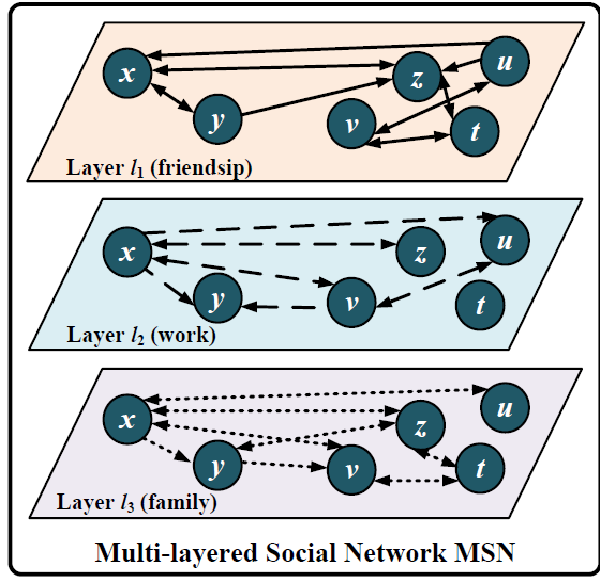
\includegraphics[width=3.8004in,height=3.6894in]{figures/chap3/chapitre3-img3.png}
    \caption [r\'eseau social multi-couches] {Un r\'eseau social multi-couches, d{\textquoteright}apr\`es (Brodka\&al., 2013)}
\end{figure}

Nous pouvons ainsi d\'ecrire diff\'erents jeux de relations entre un jeu
d{\textquoteright}acteurs finis, permettant notamment de mieux
comprendre les relations entre ses diff\'erentes dimensions. Si cette
approche r\'esout momentan\'ement la question des \textit{n }dimensions
\`a consid\'erer \cite{Br\'odka2013} elle augmente \'egalement la
complexit\'e du graphe et la possibilit\'e d{\textquoteright}erreurs de
lecture ou de typage des relations. 

Afin de mieux comprendre l{\textquoteright}organisation
d{\textquoteright}un r\'eseau, nous disposons de plusieurs mesures~pour
d\'ecrire les relations et le r\^ole des diff\'erents acteurs : 
i
\begin{itemize}
\item \textit{Degree} : (\textit{degr\'e} ou \textit{valence}) mesure le
nombre de connections d{\textquoteright}un n{\oe}ud dans un r\'eseau.
Cette valeur indique souvent une possibilit\'e, le potentiel
d{\textquoteright}un node donn\'e \`a interagir avec
d{\textquoteright}autres. 
\item \textit{Closeness : }(proximit\'e) mesure la facilit\'e
d{\textquoteright}un node \`a se connecter \`a un autre. Dans un
r\'eseau en ligne, on calcule la proximit\'e en estimant la distance la
plus courte entre un node et un autre. 
\item \textit{Betweenness} (\textit{centralit\'e}) mesure le degr\'e
d{\textquoteright}importance d{\textquoteright}un node dans le r\'eseau
en prenant en compte le nombre de nodes d\'ependant de lui pour
\'etablir une connection entre eux. La centralit\'e repr\'esente la
capacit\'e \`a bloquer ou laisser filtrer l{\textquoteright}acc\`es \`a
certaines parties du r\'eseau. Dans une entreprise par exemple, la
secr\'etaire du CEO a par exemple une tr\`es haute centralit\'e.
\end{itemize}


En observant ces diff\'erentes mesures, nous pouvons d\'efinir
diff\'erentes structures types pour chaque r\'eseau. La distribution
des degr\'es dans le graphe permet notamment de comprendre les
mod\`eles qui r\'egissent les connexions entre les nodes.
L{\textquoteright}exemple le plus simple est le \textit{random network,
}r\'eseau o\`u les acteurs sont connect\'es de mani\`ere enti\`erement
al\'eatoire. Un r\'eseau dont le degr\'e de distribution correspond \`a
une loi de puissance est appel\'e \textit{scale-free network. }Un
r\'eseau dont seulement quelques nodes poss\`edent une centralit\'e
\'elev\'ee et dont la structure d{\textquoteright}ensemble est faite de
groupes ou \textit{clusters} interconnect\'es et appel\'e un
\textit{small-world network. }


\begin{figure}
    \centering
    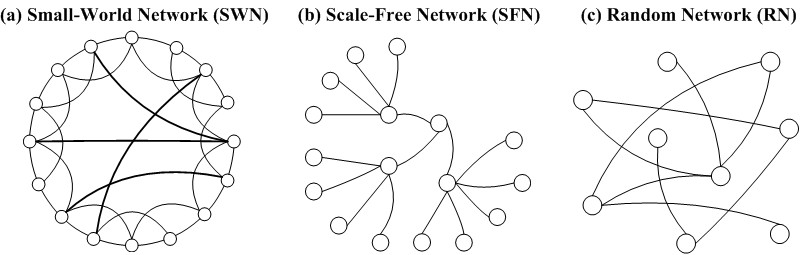
\includegraphics[width=6.3449in,height=2.0224in]{figures/chap3/chapitre3-img4.jpg}
    \centering{Types communs de r\'eseaux}
\end{figure}

Les services de r\'eseaux sociaux en ligne sont structur\'es en
\textit{small-worlds}. Dans une \'etude analysant de larges corpus
issus de diff\'erents services de r\'eseaux sociaux en ligne, Kumar \&
al. \cite{Kumar2006} ont montr\'e que ces communaut\'es poss\`edent toutes une
structure et une \'evolution similaire. Les inscrits de chaque service
se r\'epartissent autour de trois grands groupes : \textit{singletons}
(membres isol\'es, inactifs), \textit{giant component} (la majorit\'e
des utilisateurs actifs) et \textit{middle region} (des communaut\'es
isol\'ees qui interagissent entre elles mais pas avec le reste du
r\'eseau). D{\textquoteright}apr\`es les auteurs, il existe tr\`es peu
de chances que deux communaut\'es isol\'ees m\^eme tr\`es similaires se
rencontrent dans ce type de r\'eseau, car l{\textquoteright}entropie de
la structure \textit{small-world }se renforce avec le temps en se
fragmentant davantage. Une des raisons principales est que ces
communaut\'es isol\'ees suivent souvent un mod\`ele en
\textit{\'etoile, }c{\textquoteright}est \`a dire
qu{\textquoteright}elles sont construites autour d{\textquoteright}un
individu central charismatique. \'Eventuellement, il leur arrive de
rejoindre la masse du \textit{giant component} mais elles en deviennent
difficilement des acteurs majeurs et restent en p\'eriph\'erie. Dans un
r\'eseau social de type small-world comme les OSNS, les acteurs les
plus influents sont ceux qui sont capables de 1) renforcer les liens
dans un cluster (\textit{closure)} et 2) d\'evelopper les connections
faibles entre des clusters (\textit{brokerage)} (Burt, Centola, \&
Kahl, 2008). Ce {\textquotedblleft}capital social{\textquotedblright}
est inscrit dans la structure du r\'eseau social lui-m\^eme \cite{Lin1999}
et n{\textquoteright}a pas de relations avec le degr\'e du node (son
nombre de connections) \cite{Cha2010}. L{\textquoteright}individu
le plus puissant d{\textquoteright}un r\'eseau est donc celui
poss\'edant le plus grand nombre de connections \textit{potentielles,
}proches et facilement accessibles et qui b\'en\'eficie
d{\textquoteright}une place privil\'egi\'ee pour bloquer ou autoriser
l{\textquoteright}acc\`es aux autres parties du r\'eseau.
L{\textquoteright}analyse organisationnelle a notamment montr\'e
l{\textquoteright}importance capitale des secr\'etaires pour le
maintien d{\textquoteright}une bonne circulation des informations dans
le r\'eseau de l{\textquoteright}entreprise ou la n\'ecessit\'e
d{\textquoteright}un nombre tr\`es faible de connections directes pour
les acteurs importants de r\'eseaux terroristes ou mafieux \cite{Russel2011}. 

\subsection[Diffusion des discours dans les r\'eseaux sociaux]{Diffusion des discours dans les r\'eseaux sociaux}
L{\textquoteright}analyse de r\'eseau social permet de comprendre la
structure d{\textquoteright}un moment du r\'eseau. En effet, les
connections entre diff\'erents acteurs sont sans cesse en mouvement et
l{\textquoteright}information en circulant vient modifier
l{\textquoteright}activit\'e du r\'eseau et bien souvent sa structure
m\^eme. Notre \'etude porte sur la diffusion de m\`emes au sein du
r\'eseau social chinois Sina Weibo et s{\textquoteright}inscrit ainsi
dans la continuit\'e des travaux s{\textquoteright}int\'eressant aux
rapports entre diffusion et technologies. N\'eanmoins, le champ de la
diffusion de l{\textquoteright}innovation, objet traditionnel de la
g\'eographie, s{\textquoteright}est largement constitu\'e autour des
probl\'ematiques technologiques et organisationnelles li\'ees \`a la
situation spatiale du lieu et ses \'equipements \cite{Crevoisier2004}. Les
\'etudes urbaines ont notamment montr\'e comment la r\'ealit\'e
\'economique et g\'eographique pr\'esidait \`a la constitution des
savoirs n\'ecessaires \`a la diffusion de l{\textquoteright}innovation
technologique \cite{Howells2002}. Cette vision doit \^etre mod\'er\'ee par
une consid\'eration plus importante des modalit\'es
d{\textquoteright}appropriation des technologies comme pratiques
propres aux territoires \cite{Fernandez2010}. Plus largement, les
\'etudes sur la diffusion sont domin\'ees par
l{\textquoteright}analogie du virus comme mod\`ele de propagation des
messages, comportements et id\'ees. Depuis la fin du XIXe si\`ecle (Le
Bon, 1895), ce mod\`ele est pr\'epond\'erant dans les recherches autour
de la diffusion d{\textquoteright}information en ligne \cite{Goel2012} Les membres de groupes dans un r\'eseau seraient
\textit{expos\'es }\`a un message ou une id\'ee avant
d{\textquoteright}\^etre \textit{infect\'es, }devenant alors porteur
puis agent de sa diffusion. Ainsi, en consid\'erant la position
d{\textquoteright}un individu au sein du r\'eseau de diffusion, il
serait possible de d\'efinir un
\textit{{\textquotedblleft}}\textit{degr\'e
d{\textquoteright}infection{\textquotedblright}} \cite{Cheng et al.2013}
et d{\textquoteright}anticiper la diffusion selon une
\textit{{\guillemotleft}~probabilit\'e immune~{\guillemotright}
}qui\textit{ }d\'eciderait de la \textit{{\guillemotleft}~qualit\'e
infectieuse~{\guillemotright} }de l{\textquoteright}objet diffus\'e ou
de la \textit{{\guillemotleft}~possibilit\'e de
}\textit{r\'etablissement~{\guillemotright} }du sujet infect\'e \cite{Wang2011}. Cette analogie du viral propose une vision
m\'ecaniste qui fait peu de cas des facteurs contextuels ou
psychologiques et ignorent ainsi les processus de d\'ecisions
individuels en jeu \cite{Jackson2010}. Pourtant, nous savons
notamment que le choix des mots ou la situation des personnes diffusant
un message sont des facteurs d\'ecisifs et structurant des processus
d{\textquoteright}adoption des messages en ligne \cite{Conover2013}. 
En s{\textquoteright}int\'eressant \`a la diffusion
g\'eographique de mots dans les r\'eseaux sociaux, Eisenstein \& al.
\cite{Eisenstein2012} observe que leur diffusion se limite \`a un domaine
g\'eographiquement bien d\'efini, d\'ependant de facteurs culturels et
d\'emographiques. Par exemple, les villes ayant
d{\textquoteright}importantes communaut\'es afro-am\'ericaines ont
davantage de chances d{\textquoteright}adopter un m\^eme mot que
d{\textquoteright}autres parfois plus proches g\'eographiquement. Cette
question est au centre des \'etudes de marketing qui
s{\textquoteright}interrogent notamment sur l{\textquoteright}adoption
de nouvelles marques ou de slogans. Afin de d\'eterminer
statistiquement les possibilit\'es d{\textquoteright}adoption de
produits et pr\'evoir la p\'en\'etration dans un march\'e pr\'ecis, la
mod\'elisation math\'ematique des effets de r\'eseaux dans la diffusion
est souvent utilis\'e \cite{Bass1994}. Ici,
l{\textquoteright}analyse des donn\'ees des r\'eseaux sociaux est un
grand enjeu pour la prospective \'economique et
l{\textquoteright}application de ces mod\`eles math\'ematiques aux
donn\'ees utilisateurs permettant de consid\'erer des segments pr\'ecis
de march\'e. Le marketing politique fait lui aussi grand cas de
l{\textquoteright}analyse de r\'eseaux sociaux pour comprendre et
orienter les discussions. La campagne de r\'e\'election
d{\textquoteright}Obama aux USA en 2012 a fait un usage extensif de
l{\textquoteright}analyse de donn\'ees des r\'eseaux sociaux pour
identifier, d\'eterminer et cibler des groupes sociaux particuliers
gr\^ace au travail d{\textquoteright}une vaste \'equipe
d{\textquoteright}ing\'enieurs et de \textit{{\textquotedblleft}data
scientists{\textquotedblright}}\footnote{
\textit{{\textquotedblleft}Harper Reed, the chief technology officer
for the Obama re-election campaign, who heads a team described as
{\textquotedblleft}100 data scientists, developers, engineers,
analysts, and old-school hackers [that] have been transforming the way
politicians acquire data---and what they do with
it.{\textquotedblright}, }from \ The Blaze
\url{http://www.theblaze.com/stories/2012/10/03/very-creepy-details-of-obama-campaigns-voter-data-mining-effort/}
consult\'e le 12 Mars 2014 \`a 14:50 GMT+1}\textit{. }

Une des grandes interrogations dans ce domaine est \'evidemment les
r\^oles jou\'es par les diff\'erents acteurs du processus de diffusion
-- et la mani\`ere de les identifier. Les \'etudes concernant les
leaders d{\textquoteright}opinion, traditionnelles en sciences de la
communication \cite{Katz1955} trouvent une continuit\'e
directe dans l{\textquoteright}\'etude des r\'eseaux sociaux en ligne
avec le domaine florissant des recherches sur
l{\textquoteright}identification des \textit{influenceurs} \cite{Bakshy2011, Leavitt2009}. L{\textquoteright}analyse quantitative permet notamment de mieux
comprendre l{\textquoteright}influence r\'eelle des acteurs dans le
r\'eseau gr\^ace \`a l{\textquoteright}\'etude de leurs comportements.
Le concept d{\textquoteright}influence sur les r\'eseaux sociaux
rev\^et en r\'ealit\'e des formes tr\`es variables et proc\`ede
notamment d{\textquoteright}une l\'egitimit\'e construite autour de
sujets pr\'ecis par \ des personnes sp\'ecialis\'ees devenues
r\'ef\'erentes \cite{Cha2010}. D{\textquoteright}autres
{\textquotedblleft}influenceurs{\textquotedblright} poss\`edent une
grande capacit\'e d{\textquoteright}amplification pouvant par exemple
initier le d\'eveloppement d{\textquoteright}une
\textit{{\textquotedblleft}masse critique{\textquotedblright} }autour
d{\textquoteright}une information\textit{, }d\'efinie classiquement
comme le seuil d{\textquoteright}adoption \`a partir duquel la
diffusion devient p\'erenne parmi une foule d{\textquoteright}acteurs
\cite{Oliver2001}. L{\textquoteright}image quantitative
d{\textquoteright}une {\textquotedblleft}masse{\textquotedblright}
uniforme et actionnable dans le r\'eseau est n\'eanmoins remise en
question par l{\textquoteright}\'etude de donn\'ees dont
l{\textquoteright}analyse montre que les relations entre diff\'erents
acteurs du r\'eseau sont \`a consid\'erer qualitativement en termes de
relations de pouvoirs \cite{Steyer2006}\textit{. }Les dynamiques
d{\textquoteright}\'echanges ne r\'epondent en effet pas tant \`a une
relation pr\'e-existente dans le r\'eseau qu{\textquoteright}\`a un
ensemble de situations o\`u les acteurs adoptent des comportements et
des r\'eactions particuli\`eres. La diffusion peut ainsi se comprendre
comme une pratique du \textit{bouche-\`a-oreille} \'eminemment
contextuelle, o\`u certains acteurs sont plus ou moins influents dans
telle ou telle situation ou sur tel et tel sujet. Le temps joue
n\'eanmoins un r\^ole d\'eterminant puisqu{\textquoteright}en
consid\'erant des s\'eries de r\'esultats o\`u des acteurs se
c\^otoient durant plusieurs ann\'ees, il est souvent difficile
d{\textquoteright}identifier quel acteur influence
l{\textquoteright}autre \cite{Aral2009}. 

\subsection[M\'ethodes d{\textquoteright}analyse de donn\'ees des r\'eseaux sociaux en ligne]{3.2.3. M\'ethodes d{\textquoteright}analyse de donn\'ees des r\'eseaux sociaux en ligne}
Apr\`es moins d{\textquoteright}un si\`ecle d{\textquoteright}existence,
l{\textquoteright}analyse de r\'eseaux sociaux sous forme de graphes a
donc connu une rapide \'evolution et une diversification dans de
nombreux domaines de recherche. Les services de r\'eseaux sociaux en
ligne offrent notamment la possibilit\'e d{\textquoteright}obtenir des
donn\'ees sur les comportements de groupes sociaux en tr\`es vaste
quantit\'e. V\'eritable vivier d{\textquoteright}\'etudes, ce champ de
recherche en pleine expansion trouve ses origines dans des disciplines
diverses qui poursuivent souvent des objectifs et des m\'ethodes tr\`es
diff\'erentes. Le tableau infra pr\'esente quelques-unes des m\'ethodes
d{\textquoteright}analyse de donn\'ees d\'efinies selon leurs domaines
d{\textquoteright}application. Ces m\'ethodes coexistent souvent lors
d{\textquoteright}\'etudes utilisant le \textit{data mining} ; nous
pr\'esentons ici des exemples qui permettront ensuite de mieux situer
nos perspectives de recherche~dans ce paysage de pratiques.



\begin{figure}
    \centering
\caption[Tableau r\'ecapitulatif de m\'ethodes d{\textquoteright}analyse de donn\'ees de r\'eseaux sociaux en ligne.]{Tableau r\'ecapitulatif de m\'ethodes d{\textquoteright}analyse de donn\'ees de r\'eseaux sociaux en ligne.}

\begin{tabular}{c|c|c|c|c}

&
\textbf{Courant d{\textquoteright}analyse} &
\textbf{M\'ethodologie} &
\textbf{Exemples d{\textquoteright}usages et applications} &
\textbf{Auteurs \& Publications de r\'ef\'erence}\\

1 &
Graphes sociaux de groupe d\'efinis (cartographie de r\'eseau fini) &
En partant d{\textquoteright}un \'echantillon fini et d\'etermin\'e au pr\'ealable, on effectue une carte des relations entre les diff\'erents acteurs du r\'eseau.  &

Cartographier les connections d{\textquoteright}apr\`es un profil sur un service de r\'eseau social en ligne  &
Cette pratique est l{\textquoteright}origine de la sociom\'etrie (Moreno \& Jennings, 1938) et de l{\textquoteright}\'etude des relatons sociales en tant que r\'eseaux.
\\

2 &
D\'ecouverte de groupes par crit\`eres (communaut\'es)

~
 &
Cette m\'ethode permet de r\'ealiser un \'echantillonnage
d{\textquoteright}un r\'eseau social \`a partir d{\textquoteright}un
ensemble de profils existants appel\'es \textit{seeds}. Un logiciel
(appel\'e \textit{crawler}) va rechercher et collecter les profils
similaires aux \textit{seeds} selon des crit\`eres d\'efinis :
similarit\'e, diff\'erence, profondeur, etc. 

~
 &
Identifier des communaut\'es d{\textquoteright}apr\`es un type
d{\textquoteright}utilisateur t\'emoin

Trouver des profils d{\textquoteright}utilisateurs similaires
d{\textquoteright}apr\`es des profils existants &
H\'erit\'e de la tradition de l{\textquoteright}\'echantillonnage
\textit{{\textquotedblleft}boule de neige{\textquotedblright}} en
statistiques \cite{Rothenberg1995}, les algorithmes de \textit{crawling}
sont nombreux et il n{\textquoteright}existe pas de v\'eritable
consensus sur leur utilisation \cite{Gjoka2011}

~
\\
3 &
Analyse s\'emantique des conversations (analyse de contenu)

~
 &
En utilisant une masse textuelle de posts, un syst\`eme est charg\'e
d{\textquoteright}extraire et de classifier les mots et sujets
discut\'es. Ce type de syst\`eme se fonde sur l{\textquoteright}analyse
naturelle de langage (NLP) et parfois sur l{\textquoteright}analyse
structurelle des conversations \cite{Karandikar2010}.

~
 &
D\'etection de tendances dans les conversations, Reconnaissance des
entit\'es dans un texte~(\textit{semantic tagging}) : noms de lieu,
personnes, etc. &
A mi-chemin entre linguistique et informatique \cite{Russel2011}, ce champ
est un des grands enjeux actuels du Big Data \cite{Nettleton2013} avec
notamment l{\textquoteright}analyse des sentiments (Liu \& Zhang, 2012)
\\
4 &
Analyse de la diffusion 

(\'evolution des \ relations d{\textquoteright}apr\`es une conversation)
&
D{\textquoteright}apr\`es une masse de posts extraites selon des
crit\`eres pr\'ecis (souvent un mot-cl\'e ou \textit{hashtag}), il
s{\textquoteright}agit ici de retracer les dynamiques relationnelles
qui entourent ou suscitent la conversation en recr\'eant le graphe
social entourant la discussion et son \'evolution.  &
Analyse d{\textquoteright}une campagne de marketing viral

D\'etection de communaut\'es autour d{\textquoteright}un sujet pr\'ecis

D\'etection d{\textquoteright}influenceurs \cite{Cha2010}

R\^oles et partitionnement des acteurs de la diffusion (Kwak, Lee, Park,
\& Moon, 2010) &
Le mod\`ele classique du \textit{word-of-mouth }\cite{Steyer2006} et l{\textquoteright}approche
\'epid\'emiologique \cite{Wang2011} sont souvent utilis\'es
dans l{\textquoteright}analyse de la diffusion de contenus en ligne \cite{Cheng2013}.\\
5 &
Analyse comportementale et agents de diffusion (classifications et
mesures)

~
 &
Ici on \'etudie l{\textquoteright}activit\'e d{\textquoteright}un ou
plusieurs agents en analysant leur comportement dans le r\'eseau
(volume d{\textquoteright}activit\'e, fr\'equence, etc.) souvent pour
d\'efinir des crit\`eres et mesures qui permettent de classifier par
type ou d{\textquoteright}anticiper les actions d{\textquoteright}un
acteur du r\'eseau. &
D\'etection d{\textquoteright}influenceurs

Mesures de la probabilit\'e de diffusion \cite{Anagnostopoulos2012}

Typologie des utilisateurs par comportement

Effet psychologique des signaux sur un utilisateur &
Pr\'esentes notamment dans le champ du marketing \cite{Leskovec2005} et de la politique \cite{Lotan2011}, 

ce type d{\textquoteright}analyse cherche \`a comprendre et retracer les
processus parfois psychologiques \cite{Robins2013} de prise de d\'ecisions
individuelle.\\
6 &
Analyse contextuelle et g\'eographique  &
Ce type d{\textquoteright}analyse cherche \`a mettre en perspective des
facteurs ext\'erieurs au r\'eseau afin d{\textquoteright}en comprendre
l{\textquoteright}influence et les effets. Entre sciences sociales et
informatique, ce type d{\textquoteright}\'etude porte souvent sur
l{\textquoteright}usage du r\'eseau plus que sur sa structure ou son
\'evolution \cite{Torrens2010} &
Approche sociologique des usages

Mesures d{\textquoteright}impact \ g\'eographique (node locality,
geographic clustering coeficient) &
L{\textquoteright}approche contextuelle dans l{\textquoteright}analyse
de r\'eseaux restent encore un champ \`a d\'evelopper \ \cite{Adams2012}, notamment dans la consid\'eration de facteurs
g\'eographiques \cite{Graham1998, Onnela2011}, culturels \cite{Gallagher2013} ou de langage.\\
7 &
Simulation sociale &
Afin de comprendre les dynamiques en l{\textquoteright}absence de
donn\'ees ou pour anticiper une situation \`a venir, il est possible de
mod\'eliser un environnement virtuel o\`u les comportements des acteurs
sont simul\'es \cite{Macy2002}  &
Pr\'evision de tendances d{\textquoteright}apr\`es des donn\'ees
existantes

Analyse de faits dont les donn\'ees sont manquantes ou incompl\`etes &
La d\'ecouverte de m\'ethodes de mod\'elisation du contexte de
l{\textquoteright}univers de simulation \cite{Ronald2012} est un des grands enjeux o\`u
l{\textquoteright}apport de m\'ethodes ethnographiques de terrain peut
\^etre crucial \cite{Tubaro2010}\\

\end{tabular}
\end{figure}


Notre recherche choisit donc de s{\textquoteright}appuyer sur une
\'etude de cas sp\'ecifique de Sina Weibo reprenant les \'el\'ements
m\'ethodologiques de l{\textquoteright}\'etude du graphe social de la
diffusion entourant les conversations (Fig. 1-4) et
l{\textquoteright}analyse s\'emantique des sujets dominants et
sous-jacents aux conversations (Fig. 1-3). \'Egalement, nous souhaitons
amener une plus forte contextualisation des usages (Fig. 1-6) en
prenant en compte notamment les relations entre les dimensions
s\'emantique et conversationelle, mais aussi g\'eographique de
l{\textquoteright}existence des conversations.
L{\textquoteright}approche de l{\textquoteright}\'etude des donn\'ees
des SNS par les g\'eographes notamment s{\textquoteright}est
jusqu{\textquoteright}ici largement focalis\'ee sur
l{\textquoteright}analyse des \textit{geotag} et des cartes en ligne
comme principale approche m\'ethodologique \cite{Graham2011,
Poorthuis2013}, r\'eduisant consid\'erablement les
possibilit\'es d{\textquoteright}\'etude des donn\'ees de r\'eseaux
sociaux en ligne \cite{Crampton2013}. Nous souhaitons ici mettre en
perspective ces diff\'erentes dimensions afin
d{\textquoteright}enrichir le mod\`ele d{\textquoteright}\'etude. En
effet l{\textquoteright}analyse de la diffusion utilise principalement
les graphes des r\'eseaux de diffusion mettant en sc\`ene les
utilisateurs et leurs interactions en ligne. Loin
d{\textquoteright}\^etre inint\'eressant, ce type de sch\'ema est
n\'eanmoins tr\`es r\'educteur car il se fonde sur un mod\`ele
communicationel tr\`es primaire
\textit{{\textquotedblleft}\'emetteur-r\'ecepteur{\textquotedblright}
}dont on conna\^it les limites. Les travaux de Jacobson ont notamment
permis d{\textquoteright}\'etoffer ce mod\`ele en consid\'erant les
diff\'erents aspects fonctionels des actes de communication.



\begin{figure}
    \centering

    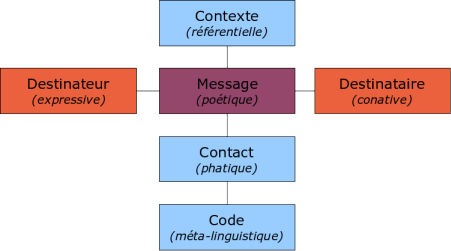
\includegraphics[width=4.6894in,height=2.6114in]{figures/chap3/chapitre3-img5.png}

    \centering[Modèle de Jakobson]{ Modèle de Jakobson, int\'eressante que nous pouvons chercher \`a adapter dans le contexte des \'echanges en ligne.}

\end{figure}

Ainsi, en nous basant sur les mod\`eles des th\'eories de la
communication, nous pouvons peut-\^etre am\'eliorer les mod\`eles
m\'ethodologiques d{\textquoteright}analyse. Nous proposons ici la
notion de \textit{topogramme }comme mod\`ele pour comprendre les motifs
de diffusion des m\`emes, consid\'er\'es comme \textit{topos} ou
\textit{lieux communs. }Le topogramme, en tant que repr\'esentation
graphique des diff\'erentes dimensions et dynamiques lisibles dans les
donn\'ees nous permet donc d{\textquoteright}approcher un travail
\ d{\textquoteright}observation pr\'ecise de la diffusion des m\`emes,
voire par la suite de classification des actes de communication en
ligne. Afin de prendre en compte, les diff\'erents aspects de la
communication, il nous faut donc effectuer une analyse \`a plusieurs
niveaux (multi-layers), regroupant un ensemble de r\'eseaux \`a la fois
s\'emantique, conversationnel et g\'eographique. 



\section{Design de la recherche : M\'ethodologie choisie et schemes d{\textquoteright}analyse retenus}

\subsection[Constitution et collection d{\textquoteright}un corpus de donn\'ees]{Constitution et collection d{\textquoteright}un corpus de donn\'ees}
Afin de poursuivre notre \'etude, nous allons donc proc\'eder \`a
l{\textquoteright}analyse de donn\'ees issues de services de r\'eseaux
sociaux en ligne. La plupart des services de r\'eseaux sociaux en ligne
offrent un large acc\`es car il s{\textquoteright}agit souvent de la
fondation de leurs mod\`eles d{\textquoteright}affaires bas\'es sur la
valorisation et la revente de ces donn\'ees pour le marketing cibl\'e
\cite{Ko2010}. Pour entrer en contact avec la base de donn\'ees, les SNS
mettent \`a disposition une API (\textit{Application Programming
Interface}) qui permet \`a un programme ou une autre application web de
se connecter au service pour demander et obtenir des donn\'ees.
L{\textquoteright}API est donc la premi\`ere source
d{\textquoteright}obtention de donn\'ees depuis les SNS. N\'eanmoins,
les donn\'ees des r\'eseaux sociaux sont soumises \`a
d{\textquoteright}importants enjeux et contraintes tant commerciales,
\'ethiques que politiques dans le cas de la Chine notamment. Les
conditions d{\textquoteright}utilisations techniques et l\'egales
(\textit{Terms of Uses) }de ces donn\'ees sont \'egalement soumises \`a
des changements fr\'equents, \'etroitement li\'es \`a
l{\textquoteright}\'evolution commerciale et technologique de
compagnies souvent tr\`es jeunes. Voici une liste des limitations et
\'ecueils pouvant \^etre rencontr\'es lors de
l{\textquoteright}extraction et de l{\textquoteright}analyse de
donn\'ees des SNS :
ii
\begin{itemize}
\item \textit{Compatibilit\'e }: Une solution technologique devient
facilement caduque lors de l{\textquoteright}\'evolution
d{\textquoteright}une API (ex. Twitter APi v1.0
n{\textquoteright}existe plus, ainsi le code doit \^etre r\'e\'ecrit
pour la version 1.1). 
\item \textit{Disponibilit\'e des donn\'ees :} Chaque API r\'epond \`a
des formats et crit\`eres pr\'ecis et poss\`ede ses propres
limitations. Pour acc\'eder \`a l{\textquoteright}API du moteur de
recherche de Sina Weibo, il faut s{\textquoteright}identifier aupr\`es
de la compagnie gr\^ace \`a une carte d{\textquoteright}identit\'e et
des paiements par requ\^ete sont exig\'es. 
\item \textit{Limitations d{\textquoteright}usage : }Afin de limiter le
trafic et conserver le contr\^ole sur les donn\'ees distribu\'ees, les
SNS mettent en place des limitations d{\textquoteright}acc\`es \`a
leurs serveurs, notamment : limitation du nombre de requ\^etes par
heure, limitation du nombre de requ\^etes par machine (bas\'ee sur
l{\textquoteright}addresse IP), limitation du nombre
d{\textquoteright}utilisateurs connect\'es. Ainsi, Twitter limite \`a
150 requ\^etes API par heure pour un compte non identifi\'e, pouvant
augmenter jusqu{\textquoteright}\`a 500 apr\`es authentification. Les
donn\'ees datant de plus de 7 jours sont payantes, refl\'etant la
valeur d{\textquoteright}un acc\`es en
{\textquotedblleft}temps-r\'eel{\textquotedblright} aux donn\'ees.
\item \textit{L\'egalit\'e }: Les donn\'ees sont soumises aux conditions
de propri\'et\'e d\'ecrites l\'egalement par la firme qui les publient
\cite{Clifton2006}. Ces conditions sont susceptibles de changer. Ainsi,
Twitter a exig\'e en 2012 le retrait a posteriori de nombreux jeux de
donn\'ees publi\'es par des chercheurs depuis plusieurs ann\'ees
parfois \cite{McCreadie2012}. Actuellement, Twitter pr\'ecise notamment
dans ses \textit{Terms of Use: {\textquotedblleft}You may not
resyndicate or share Twitter content, including datasets of Tweet text
and follow relationships{\textquotedblright} }\footnote{ Terms of use
de Twitter, \url{https://dev.twitter.com/terms/api-terms}, consult\'e
le 12 Mars 2013 \`a 17h08}\textit{. ~}
\item \textit{Ethique : }Vous pouvez extraire depuis une API des profils
d{\textquoteright}utilisateurs contenant les informations
qu{\textquoteright}ils ont auparavant publi\'e en ligne (Felt \& Evans,
2008). En exposant les donn\'ees personnelles des utilisateurs, le
chercheur est responsable de l{\textquoteright}usage
qu{\textquoteright}il fait des donn\'ees \cite{Rieder2005} 
\end{itemize}
Afin d{\textquoteright}obtenir des donn\'ees et de contourner les
limitations de l{\textquoteright}API, la pratique dite du
\textit{{\textquotedblleft}scraping{\textquotedblright} }permet
d{\textquoteright}obtenir des donn\'ees \`a l{\textquoteright}aide
d{\textquoteright}un robot qui lit et sauvegarde des parties ou
l{\textquoteright}int\'egralit\'e de pages web. Les moteurs de
recherche utilisent notamment cette technique pour
l{\textquoteright}indexation des pages. Ce type de pratiques est
\'egalement soumis \`a des limitations par les services web (blocage de
l{\textquoteright}IP source) et se situe \`a la limite de la
l\'egalit\'e,voire est explicitement interdite dans le cas de certains
SNS \cite{Petschulat2010}.

Un programme appel\'e \textit{spider }ou \textit{crawler} est charg\'e
d{\textquoteright}effectuer des requ\^etes r\'eguli\`eres \`a
l{\textquoteright}API afin d{\textquoteright}obtenir et collecter les
informations obtenues dans une base de donn\'ees. Plusieurs approches
existent dans les techniques \'echantillonnage de r\'eseau social. La
premi\`ere, fond\'ee sur des mots-cl\'es extraits les posts contenant
des mots ou des hashtags particuliers. La seconde utilise
l{\textquoteright}\'echantillonnage de graphe, collectant au fil des
liens les conversations ou profils des utilisateurs. Classique des
\'etudes statistiques, cet \'echantillonage dit \textit{boule de neige
{\textquotedblleft}\'elargit l{\textquoteright}\'echantillon en partant
d{\textquoteright}un node original pour s{\textquoteright}\'eloigner
vers ses voisins{\textquotedblright}} \cite{Rothenberg1995}. Ici, deux
grandes cat\'egories s{\textquoteright}opposent : les techniques
traversales o\`u les nodes sont classifi\'es apr\`es avoir \'et\'e
visit\'es et les {\textquotedblleft}walk{\textquotedblright}
al\'eatoires o\`u l{\textquoteright}extension du graphe visit\'e se
fait de mani\`ere al\'eatoire \cite{Gjoka2011}. 

Au cours du travail pr\'eparatoire de cette recherche, nous avons tout
d{\textquoteright}abord exp\'eriment\'e plusieurs algorithmes et outils
de collection de donn\'ees afin d{\textquoteright}en comparer les
r\'esultats. Une premi\`ere approche d{\textquoteright}extraction par
utilisateurs a \'et\'e infructueuse car la s\'election du groupe source
(\textit{seeds}) ne permettait pas d{\textquoteright}obtenir des
r\'esultats coh\'erents\footnote{ Code disponible :
\url{https://github.com/sharismlab/Pyweibo}, consult\'e le 14 Mars \`a
5h32}. Par la suite, une autre approche de collecte de donn\'ees via le
d\'eveloppement d{\textquoteright}un plug-in pour le navigateur Google
Chrome\footnote{ Code disponible :
\url{https://github.com/sharismlab/battlefield}, consult\'e le 14 Mars
\`a 5h12\par } nous a permis de tester et d{\textquoteright}apercevoir
les limites de la collection de donn\'ees par mots-cl\'es. Cette
\'etape nous a \'egalement montr\'e l{\textquoteright}int\'er\^et que
peut pr\'esenter une approche collaborative de la collection de
donn\'ees ou de seeds par un syst\`eme de
{\textquotedblleft}curation{\textquotedblright} collaboratifs afin
d{\textquoteright}obtenir des \'el\'ements pr\'ecis de contenus et de
r\'eduire la masse de donn\'ees inutiles qui pollue souvent les jeux de
donn\'ees \cite{Ding2013}. Apr\`es de multiples tests et
comparaisons d{\textquoteright}outils et de librairies, plusieurs
difficult\'es majeures limitaient l{\textquoteright}obtention
d{\textquoteright}une quantit\'e de donn\'ees suffisantes, notamment la
n\'ecessit\'e de ressources assez importantes (en terme de
d\'eveloppement et de disponibilit\'e des machines), un temps
d{\textquoteright}acquisition parfois tr\`es long et
l{\textquoteright}exigence d{\textquoteright}une veille constante sur
les SNS pour identifier un m\`eme au bon moment (les tweets de Sina
Weibo devenant indisponibles via l{\textquoteright}API au-del\`a de 7
jours). La premi\`ere limite se situe bien s\^ur dans la capacit\'e
d{\textquoteright}une personne seule \`a mener \`a bien cette large
t\^ache. Nous avons donc choisi de consid\'erer les jeux de donn\'ees
collect\'es sur Sina Weibo disponibles sur l{\textquoteright}Internet.
Une fois \'ecart\'es les nombreux jeux tronqu\'es, modifi\'es ou
incomplets, nous avons pu obtenir plusieurs jeux de donn\'ees provenant
de recherches pr\'ealables dans le domaine particulier de
l{\textquoteright}\'echantillonnage \cite{Ding2013} ou ayant servi
de bases \`a des \'etudes pr\'ec\'edentes \cite{Gao2012, Leiden2010}. Finalement, nous avons identifi\'e le jeu de donn\'ees
constitu\'e lors du projet \textit{Weiboscope }de
l{\textquoteright}Universit\'e de Hong Kong comme r\'epondant \`a nos
besoins en termes de dimensions (temps, nombre
d{\textquoteright}utilisateurs observ\'es), taille (nombre de tweets)
et contenus (g\'eo-localisation, pr\'esence des tweets censur\'es).



Notre travail d{\textquoteright}analyse s{\textquoteright}appuie donc
sur ce jeu de donn\'ees collect\'e sur le service de microblog Sina
Weibo par le \textit{Journalism and Media Studies Centre} (JMSC) de
l{\textquoteright}Universit\'e de Hong Kong lors de son projet
\textit{Weiboscope}. T\'el\'echargeable ouvertement, la publication de
ce jeu de donn\'ees a pour objectif de
\textit{{\textquotedblleft}enables academic use of the data for better
understanding of the social }\textit{media in China and making the
Chinese media system more transparent.{\textquotedblright}}\footnote{
Le jeu de donn\'ees Weiboscope est disponible \`a l{\textquoteright}adresse :
\url{http://147.8.142.179/datazip/}, consult\'e le 14 Mars \`a 17h21 }\textit{ }Il s{\textquoteright}agit
d{\textquoteright}un \'echantillonnage al\'eatoire de messages
\textit{(random sampling)} effectu\'e quotidiennement durant toute
l{\textquoteright}ann\'ee 2012 sur un panel d{\textquoteright}environ
350 000 utilisateurs ayant au moins 1000 followers \cite{Fu2013}. La totalit\'e du jeu de donn\'ees comprend 226,841,122 messages
r\'epartis sur 52 semaines, dont des messages ayant \'et\'e supprim\'es
par les utilisateurs eux-m\^emes ou par les administrateurs de Sina
Weibo eux-m\^emes - parfois sur ordre du gouvernement chinois
(\textit{ibid}, 2013).

\begin{figure}
    \centering
    \begin{tabular}{c|c}
        mid  &
        Unique pseudo message ID\\
        retweeted\_status\_mid  &
        Pseudo message ID of the original message (Only available if the row of
        interest is a retweet)\\
        Uid &
        Pseudo user ID\\
        retweeted\_uid &
        Pseudo user ID of the original poster (Only available if the row of
        interest is a retweet)\\
        Source &
        The application name of the client program\\
        Image &
        With image? (1= Yes, 0=No)\\
        text  &
        body of the message. Any address handle (@xxxx:) is replaced by either
        the pseudo user ID or ukn (uknown)\\
        geo &
        GIS information. Please refer to the Sina Weibo API documentation:
        \url{http://goo.gl/Um8SS}\\
        created\_at &
        Original posting time\\
        deleted\_last\_seen &
        The last seen time before this message was missing from the user
        timeline\\
        permission\_denied  &
        {\textquotesingle}permission denied{\textquotesingle} status is marked
        when the message was found missing in the timeline and the API return
        message was {\textquotesingle}permission denied{\textquotesingle} - See
        details in (Fu, Chan, Chau 2013)\\
    \end{tabular}
 \end{figure}





Ce jeu de donn\'ees a \'et\'e mis \`a disposition sous une forme
anonymis\'ee o\`u les identifiants des messages et des utilisateurs ont
\'et\'e remplac\'es par des pseudo-identifiants. La collection des
donn\'ees a \'et\'e effectu\'ee sur une s\'erie
d{\textquoteright}utilisateurs (g\'en\'eration al\'eatoire
d{\textquoteright}identifiants dont l{\textquoteright}existence est
ensuite valid\'ee) pour donner \textit{{\textquotedblleft}une image
repr\'esentative des usages et utilisateurs de Sina Weibo (...) dont
les \'etudes auparavant limit\'ee \`a des analyses non-al\'eatoire
(...) se cantonnaient aux utilisateurs les plus
populaires{\textquotedblright} }\cite{Fu2013}. Ainsi, plut\^ot que
de consid\'erer uniquement les
{\textquotedblleft}stars{\textquotedblright} de Sina Weibo, cet
\'echantillon s{\textquoteright}attache \`a refl\'eter \'egalement les
pratiques des utilisateurs
{\textquotedblleft}lambda{\textquotedblright}. Ce jeu de donn\'ees a
d\'ej\`a \'et\'e partiellement \'etudi\'e dans le but de comprendre la
d\'emographie des utilisateurs de Sina Weibo, leurs activit\'es et les
comportements pouvant permettre de pr\'edire les r\'eactions notamment
de censure \cite{Fu2013}. La d\'emographie des utilisateurs se
composent de 55\% d{\textquoteright}hommes habitant principalement dans
les grandes villes de Chine (P\'ekin, Canton, Shanghai). Une des
d\'ecouvertes importantes est le tr\`es faible taux de cr\'eation
originale de messages malgr\'e une activit\'e importante des
utilisateurs, indiquant que l{\textquoteright}essentiel de
l{\textquoteright}activit\'e sur Sina Weibo se constitue de re-posts et
de commentaires. Le jeu de donn\'ees est accompagn\'e des informations
succintes de profil des utilisateurs dont le lieu, rempli par eux, sans
n\'eanmoins fournir leurs noms d{\textquoteright}utilisateur
v\'eritables. Notre travail de recherche s{\textquoteright}articule
autour d{\textquoteright}une nouvelle lecture de ce jeu de donn\'ees
unique.

\subsection[Identification des m\`emes en tant que {\textquotedblleft}clusters{\textquotedblright}]{Identification des m\`emes en tant que {\textquotedblleft}clusters{\textquotedblright}}
Une fois l{\textquoteright}acquisition des donn\'ees effectu\'ees, il
s{\textquoteright}agit d\'esormais de savoir les analyser correctement
pour y d\'eceler les m\`emes que nous souhaitons consid\'erer. Les
travaux dans le domaine de la d\'etection et
l{\textquoteright}identification de m\`emes dans les donn\'ees de
r\'eseaux sociaux restent encore peu nombreux. Une des \'etudes
pionni\`eres est l{\textquoteright}outil \textit{MemeTracker }(devenu
\textit{NIFTY}) con\c{c}u en 2009 par le \textit{SNA Project }de
l{\textquoteright}Universit\'e de Stanford \cite{Leskovec2009}. Cet
outil permet une \'etude sous forme de graphes de la diffusion de
phrases dans un vaste corpus de texte mais n{\textquoteright}est pas
adapt\'e \`a la langue chinoise. La discussion sur la mod\'elisation
math\'ematiques des m\`emes \cite{Ahmad2006, Nye2011} \'emane souvent
de recherches en informatique cherchant \`a prendre en consid\'eration
diff\'erents facteurs de diffusion lors de l{\textquoteright}analyse
machine de donn\'ees \cite{Zubiaga2011, Wang2011)},
consid\'erant le m\`eme comme un vecteur de modification du r\'eseau
lui-m\^eme \cite{Ienco2010}. Plus marginal, des \'etudes
s{\textquoteright}int\'eressent aux dynamiques g\'eographiques des
m\`emes \cite{Kamath2013}. N\'eanmoins, aucune de ces diff\'erentes
approches ne permet d{\textquoteright}apporter une r\'eponse
technologique ou algorithmique satisfaisante pour
l{\textquoteright}identification de m\`emes Internet dans un ensemble
de donn\'ees issu des r\'eseaux sociaux. Afin de d\'eceler les m\`emes
dans un vaste ensemble textuel, nous devons y d\'eceler des motifs de
diffusion particuliers. La d\'enomination \textit{machine learning
}regroupe un ensemble d{\textquoteright}algorithmes qui permettent
d{\textquoteright}explorer des jeux de donn\'ees pour en extraire des
repr\'esentations et y identifier des propri\'et\'es
(\textit{features}) particuli\`eres. Bas\'e sur les sciences
statistiques, ces algorithmes font usage de mesures de similarit\'e
pour classifier les \'el\'ements d{\textquoteright}un corpus. Les
cat\'egories utilis\'ees pour la classification peuvent \^etre
d\'efinies au pr\'ealable par l{\textquoteright}utilisateur -
c{\textquoteright}est le \textit{{\textquotedblleft}supervised
learning{\textquotedblright} }ou inf\'er\'ees du jeu de donn\'ees
lui-m\^eme dans le cas du \textit{{\textquotedblleft}unsupervised
learning{\textquotedblright}} pour la d\'etection de \textit{clusters
}\cite{Breiman2001}\textit{. }La multitude d{\textquoteright}algorithmes
de \textit{machine learning }disponibles pour la d\'etection de
clusters au sein d{\textquoteright}un corpus textuel ou
d{\textquoteright}un r\'eseau social \cite{Nettleton2013, Robbins2013}
rend l{\textquoteright}identification d{\textquoteright}une solution
difficile. De plus, les algorithmes utilis\'es traditionnellement pour
l{\textquoteright}analyse de documents textuels (\textit{topic
modeling, LSA}) se heurtent au caract\`ere tr\`es disparate des corpus
issus des r\'eseaux sociaux (\textit{text sparsity issue) }faisant
diminuer drastiquement leur efficacit\'e \cite{Hong2010}. 



Ferrara \& al. \cite{Ferrara2013} propose dans un papier intitul\'e
{\textquotedblleft}\textit{Meme clustering in social
media}{\textquotedblright} un algorithme utilisant la classification
automatique non-supervis\'ee pour d\'etecter des m\`emes dans un corpus
de donn\'ees de r\'eseaux sociaux. Ce travail r\'ecent propose de tenir
compte non seulement des textes et hashtags, mais aussi des liens et
des mod\`eles de diffusion pour identifier des groupes de messages
int\'eressants et proc\'eder au \textit{clustering }des m\`emes.
L{\textquoteright}algorithme s{\textquoteright}articule autour du
concept de {\textquotedblleft}protom\`emes{\textquotedblright},
repr\'esentant les \'el\'ements fondamentaux d{\textquoteright}un
m\`eme en cours de cr\'eation \cite{Gabora1997}. Dans le contexte des
m\'edias sociaux, le protom\`eme est d\'efini par les entit\'es (liens,
hashtags...), mots-cl\'es et s\'equences de conversation qui constitue
le m\`eme en devenir. En identifiant puis comparant les diff\'erents
protom\`emes pr\'esents dans chaque tweet, il est possible
d{\textquoteright}y d\'etecter des similarit\'es et de deviner les
m\`emes en formation. 

\begin{figure} 
    \centering

    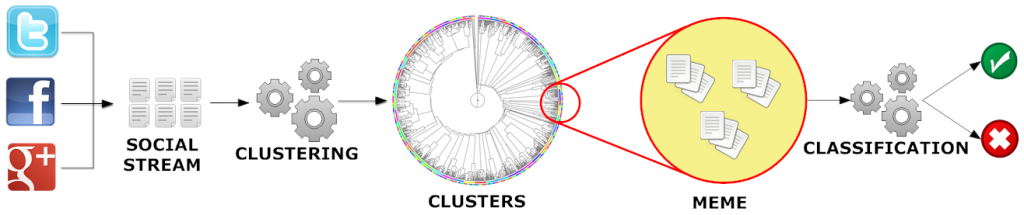
\includegraphics[width=5.8894in,height=1.2114in]{figures/chap3/chapitre3-img6.png}
    \caption{Algorithme de reconnaissance de mème (clustering) \cite{Ferrara2013}}
\end{figure}

Cet algorithme suppose donc d{\textquoteright}extraire dans un premier
temps les \'el\'ements remarquables du corpus de tweets afin
d{\textquoteright}\'etablir des repr\'esentations de ces protom\`emes
contenant les \'el\'ements \`a comparer : \textit{phrases} (texte
brut), \textit{mentions }(@, RT), \textit{hashtags }et \textit{urls}.
Pour constituer ces jeux de protom\`emes, nous utilisons le pattern
\textit{map-reduce} qui permet de chercher et lister des \'el\'ements
dans un vaste jeu de donn\'ees \textit{(map)} avant de les regrouper
dans une liste \textit{(reduce)}. Une fois ces protom\`emes
constitu\'es nous proc\'edons \`a leurs comparaisons selon plusieurs
crit\`eres :
v
\begin{itemize}
\item \textit{Similarit\'e de texte }: comparant le contenu texuel de
chaque protom\`eme 
\item \textit{Similarit\'e d{\textquoteright}utilisateurs} : comparant
les utilisateurs contenus dans chaque protom\`eme
\item \textit{Similarit\'es de tweet }: recherchant les tweets
identiques dans diff\'erents protom\`emes
\item \textit{Similarit\'e de diffusion : }consid\'erant les
r\'ef\'erences aux utilisateurs contenus dans chaque protom\`eme
\end{itemize}
Ici nous utilisons la \textit{s\'emantique vectorielle} (Support Vector
Machine) afin de comparer les \'el\'ements des protom\`emes gr\^ace \`a
une repr\'esentation alg\'ebrique sous formes de vecteurs. Pratique
ancienne de l{\textquoteright}alg\`ebre lin\'eaire appliqu\'ee \`a la
science informatique \cite{Salton1975}, il s{\textquoteright}agit de
permettre la conversion d{\textquoteright}objets textuels (mots,
identifiants, images...) sous une forme ais\'ement comparable. Pour
convertir le texte sous forme vectorielle, l{\textquoteright}algorithme
classique Tf-idf (\textit{Term Frequency - Inverse Document Frequency})
est utilis\'e \cite{Soucy2005}. Les autres mesures de similarit\'e sont la
\textit{mesure cosine (}ou \textit{similarit\'e cosinus) }des
protom\`emes convertis sous forme de vecteurs binaires. Une fois ces
diff\'erentes valeurs de similarit\'e calcul\'ees, nous utilisons les
scalaires d\'efinis dans le papier de r\'ef\'erence pour assigner des
poids \`a chacun des vecteurs et les combiner en une seule valeur
\cite{Ferrara2013}. Cette matrice de valeurs de similarit\'e nous permet
alors de d\'efinir les protom\`emes les plus similaires et
d{\textquoteright}identifier ainsi des \textit{clusters }dans les
donn\'ees correspondant aux m\`emes.



Si cette approche offre des r\'esultats probants sur de petits volumes
(quelques centaines de tweets), la tr\`es grande demande en puissance
de calcul et ressources m\'emoires n\'ecessaires rendent le traitement
d{\textquoteright}un jeu donn\'ees plus vaste irr\'ealisable. Les
op\'erations de comparaison et le calcul de similarit\'es sur de vastes
volumes de donn\'ees font cro\^itre tr\`es rapidement la complexit\'e
des algorithmes et ainsi la quantit\'e de calculs \`a effectuer. Le
calcul du co\^ut d{\textquoteright}un algorithme se fait au travers des
notions dites de domination, avec notamment le {\textquotedblleft}grand
O{\textquotedblright} exprim\'e \textit{O(f(n)) }qui fait correspondre
\`a la complexit\'e d{\textquoteright}un algorithme une fonction
\textit{f} de la quantit\'e d{\textquoteright}information manipul\'ee
\textit{n. }Ainsi pour un algorithme courant de complexit\'e
\textit{O(n}\textit{\textsuperscript{2}}\textit{), }les ressources de
calcul \textit{(computation)} et de m\'emoire (RAM ou stockage)
n\'ecessaires augmentent de mani\`ere exponentielle \`a chaque
\'el\'ement ajout\'e au corpus \textit{n}. L{\textquoteright}algorithme
de {\textquotedblleft}meme clustering{\textquotedblright} d\'ecrit par
Ferrara atteint donc un co\^ut exorbitant devant un large volume de
donn\'ees comme celui du jeu Weibosope. La limite physique de calcul
est rapidement atteinte rendant impossible le franchissement du pallier
exp\'erimental et la v\'erification des hypoth\`eses de travail \`a une
\'echelle suffisante.

\subsection[ L{\textquoteright}identification des m\`emes par hashtags ]{L{\textquoteright}identification des m\`emes par hashtags }
Les travaux en sciences humaines sur les m\`emes \cite{Bauckhage2011,
Coscia2013, Knobel2007} et les sites sp\'ecialis\'es \cite{Buchel2012, Bernstein2011} pr\'esente bien souvent un m\`eme sous la forme
d{\textquoteright}un titre (mot ou groupe de mots) accompagn\'e
d{\textquoteright}une collection d{\textquoteright}images ou/et de
vid\'eos, ainsi qu{\textquoteright}un texte explicatif (mise en
contexte) et des indications sur les dates de parution et son
\'evolution dans le temps. Ici, un ou des auteurs se saisissent des
mat\'eriaux bruts du web et les rassemblent pour reconstituer une
vision particuli\`ere du m\`eme, aussi repr\'esentative que possible.
Cette approche n\'ecessite peu de d\'eploiement technologique (un
copier/coller suffit souvent), mais exige n\'eanmoins une forte
connaissance et un suivi r\'egulier du terrain Internet pour y
d\'enicher ces repr\'esentations du m\`emes. Cette d\'emarche que nous
nommerons \textit{ethnographique }s{\textquoteright}apparente \`a de la
curation de contenu \cite{Buckingham2006}. Les \textit{hashtags }(en
fran\c{c}ais {\textquotedblleft}mots-di\`eses{\textquotedblright}) sont
utilis\'es dans l{\textquoteright}\'ecriture sur les r\'eseaux sociaux
et se pr\'esentant dans Sina Weibo sous la forme d{\textquoteright}un
mot entour\'e de deux di\`eses - ex. \textit{\#mot-cl\'e\#}. Marqueur
particulier, le hashtag permet \`a un interlocuteur de proc\'eder \`a
une d\'enotation ou connotation du message original \cite{Romero2011} ou
d{\textquoteright}affirmer son caract\`ere \'ev\`enementiel (lors
d{\textquoteright}un \'ev\`enement sportif, d{\textquoteright}une
conf\'erence, etc). Facile \`a identifier dans la masse des donn\'ees
en ligne, il permet de d\'esigner un ensemble de contenus sous un
m\^eme signe. Ainsi, il est un vecteur important permettant de
collecter simplement une large masse d{\textquoteright}informations
autour d{\textquoteright}un m\`eme. La constitution
d{\textquoteright}un corpus autour d{\textquoteright}un
{\textquotedblleft}hashtag{\textquotedblright} pr\'esente n\'eanmoins
plusieurs limites. Premi\`erement, le m\`eme est par d\'efinition un
objet en mutation. Ainsi, il est souvent difficile de
l{\textquoteright}identifier une bonne fois pour toute par un ou
plusieurs de mot-cl\'es. De plus, le m\`eme existe bien souvent sous la
forme d{\textquoteright}images ou de vid\'eos qui ne sont pas
n\'ecessairement l\'egend\'ees ou r\'ef\'erenc\'ees et donc peu
accessible \`a une recherche {\textquotedblleft}plein
texte{\textquotedblright}. Ainsi, une approche pour la recherche de
m\`emes ne peut \^etre enti\`erement textuelle et doit
s{\textquoteright}int\'eresser aux autres forme de contenus web
(notamment les liens et les hashtags). De plus, l{\textquoteright}ajout
de hashtags dans les messages est un acte volontaire non
syst\'ematique. Ainsi, si l{\textquoteright}identification de certains
m\`emes peut se faire gr\^ace \`a la recherche de hashtags,
l{\textquoteright}ensemble des messages contenant des hashtags ne
recouvrent pas syst\'ematiquement un m\`eme. Comme nous le verrons, les
hashtags sont bien souvent de simples artefacts de campagne marketing
en ligne.



Afin de proc\'eder \`a l{\textquoteright}analyse des m\`emes, nous avons
donc index\'e l{\textquoteright}ensemble des contenus du corpus
Weiboscope contenant des hashtags sur toute l{\textquoteright}ann\'ee
2012 (30 millions sur un total de 200 millions tweets environs). Nous
avons donc dans un premier temps extrait l{\textquoteright}ensemble des
messages contenant un ou des hashtags de l{\textquoteright}ensemble des
donn\'ees avant de les classifier pour obtenir des jeux de donn\'ees
coh\'erents par hashtags. Une premi\`ere contrainte ici est propre au
traitement informatique de la langue chinoise qui constitue le langage
majoritaire de notre corpus. L{\textquoteright}absence
d{\textquoteright}espace entre les diff\'erents caract\`eres de la
phrase en chinois oblige \`a prendre en compte la s\'emantique de la
phrase pour proc\'eder \`a sa segmentation. Cette question usuelle pour
les usagers du NLP (\textit{Natural Language Processing}) en chinois
est un sujet de recherche encore tr\`es discut\'e \cite{Qiu2013}.
L{\textquoteright}identification de la meilleure option parmi la
multitude des librairies et logiciels disponibles pour la segmentation
puis le NLP en chinois a \'et\'e un aspect pr\'eliminaire importants de
notre travail d{\textquoteright}analyse de donn\'ees. Nous avons ainsi
r\'ealis\'e de nombreux benchmark afin de comparer les diff\'erentes
technologies existantes. Un travail men\'e avec
l{\textquoteright}\'equipe du site Internet
d{\textquoteright}actualit\'e scientifique \textit{Guokr }\`a P\'ekin
nous a amen\'e \`a choisir en premier lieu un algorithme de
segmentation d\'evelopp\'e sur la base de textes en chinois
ancien\footnote{ gkSeg : \textit{{\textquotedblleft}Yet another Chinese
word segmentation package based on character-based tagging heuristics
and CRF algorithm{\textquotedblright}
}\url{https://github.com/guokr/gkseg}, consult\'e le 14 Mars \`a
18:28}. Apr\`es plusieurs tentatives, nous avons pr\'ef\'er\'e le
segmenteur open-source Jieba\footnote{
\url{https://github.com/fxsjy/jieba}, consult\'e le 14 Mars \`a 18:30}
plus g\'en\'ereux en termes de fonctionnalit\'es et permettant de
meilleures performances. Une fois la phrase chinoise segment\'ee, la
seconde \'etape consiste \`a supprimer tous les mots les plus communs
\textit{(stopwords)}, ainsi que la ponctuation et
d{\textquoteright}autres caract\`eres trop courants afin de pr\'eserver
uniquement les mots riches de sens dans les phrases (les mots-cl\'es).
L{\textquoteright}extraction des hashtags est effectu\'ee gr\^ace \`a
une expression r\'eguli\`ere qui scanne le texte pour identifier et
pr\'eserver uniquement les caract\`eres situ\'es entre les deux signes
di\`ese (\#). Sur un total d{\textquoteright}environ 30 millions de
tweets contenant des hashtags, nous avons choisi de retenir seulement
les hashtags poss\'edant plus de 1000 messages. Nous avons ensuite
d\'ecid\'e d{\textquoteright}ignorer les 1000 hashtags les plus
utilis\'es car ils ne pr\'esentaient pas d{\textquoteright}int\'er\^et
pour notre \'etude, \'etant la plupart du temps des noms de marque ou
des mots-cl\'es trop g\'en\'eraux (par exemple :
{\textquotedblleft}bonne nuit{\textquotedblright},
{\textquotedblleft}nouvelles de sports{\textquotedblright},
{\textquotedblleft}photos de nourriture{\textquotedblright}, etc.) 


\begin{figure}
    \centering
    
    \subfloat[Hashtags les plus utilis\'es pendant la 1\`ere semaine de 2012] {
        \begin{tabular}{c|c|c|c}
            hashtags & users &  actions & tweets \\
            \zh{吴奇隆} 201 & 13243 & 22349  \\
            \zh{一起到老} 182 & 0 & 364  \\
            \zh{春运} 92 & 13 & 256  \\
            \zh{轻松一刻} 92 & 11 & 240  \\
            \zh{人品值分析} 90 & 490 & 321  \\
            \zh{朝阳区} 88 & 49 & 165  \\
            \zh{理性态小度} 87 & 0 & 329  \\
            \zh{美图GIF} 87 & 101 & 404  \\
            \zh{我正在听} 86 & 6 & 330  \\
            \zh{微盘签到} 84 & 304 & 305  \\
            \zh{2012来了} 83 & 206 & 309  \\
            \zh{中级达人} 83 & 0 & 159  \\
            \zh{分享} 82 & 87 & 563  \\
            \zh{星座} 82 & 5 & 195  \\
            \zh{极速互联随我行} 81 & 317 & 701  \\
            \zh{微信} 80 & 11 & 288  \\
            \zh{微博达人} 80 & 9 & 364  \\
            \zh{2012} 79 & 37 & 270  \\
            \zh{那些年} 79 & 106 & 217  \\
            \zh{晚安心语} 78 & 27 & 150  \\
            \zh{周杰伦} 77 & 130 & 286  \\
            \zh{多多cosplay} 15 & 414 & 463  \\
        \end{tabular}
    }

    \subfloat[Volume de tweets pendant la semaine ]{
        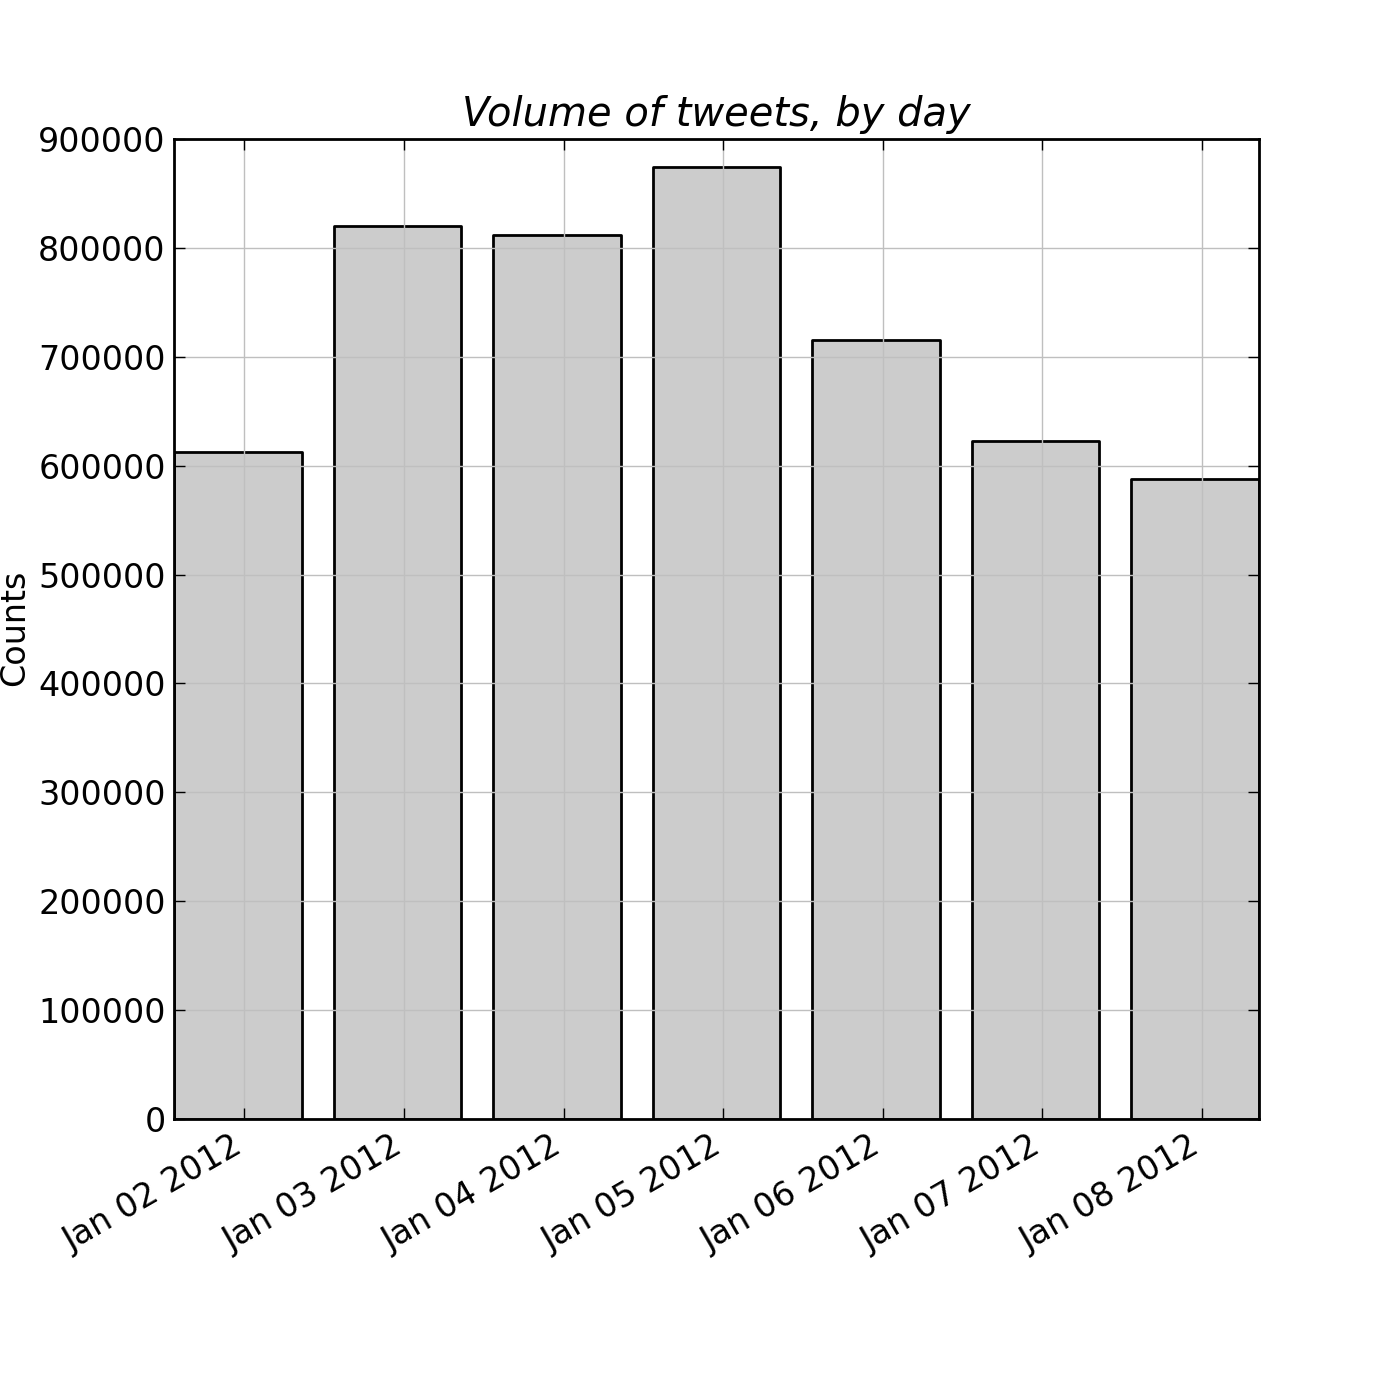
\includegraphics[width=3.2004in,height=3.2004in]{figures/chap3/chapitre3-img7.png}
    }

    \caption[Volume de tweets et hashtags pour la semaine 1]{Les r\'esultats concernant la 1\`ere semaine de l{\textquoteright}ann\'ee 2012 donnent un aper\c{c}u du volume analys\'e : 5,044,331 tweets, 398 392 utilisateurs uniques cit\'es (dans un total de 2 115 544 mentions), 264 651 urls uniques (pour un total de 426 914) et 44 382 hashtags uniques (pour un total de 244285).}
\end{figure}



Notre \'etude vise\`a \'etudier les dynamiques conversationnelles et
nous devons donc d\'eterminer les plus ad\'equats parmi des hashtags de
nature souvent tr\`es diff\'erentes. Pour ce faire, nous avons
s\'electionn\'e pour chaque jeu de donn\'ees (chaque hashtag) deux
mesures significatives : premi\`erement, le volume de messages ;
deuxi\`emement, la quantit\'e d{\textquoteright}\'echanges et
d{\textquoteright}interactions effectives entre les utilisateurs
(commentaires, retweets, etc.). Ces deux mesures nous permettent de
nous assurer que 1) nous poss\'edons une quantit\'e suffisante de
messages pour mener \`a bien l{\textquoteright}\'etude et que 2) la
discussion a bien eu lieu et qu{\textquoteright}il ne
s{\textquoteright}agit pas de messages redondants ou non reli\'es entre
eux. Nous avons choisi d{\textquoteright}ignorer les \'echanges
domin\'es \`a plus de 80\% par le m\^eme utilisateur pour \'eviter la
pollution de l{\textquoteright}\'etude par l{\textquoteright}activit\'e
de robots. Le graphe ci-dessous permet d{\textquoteright}observer la
distribution de 429 hashtags poss\'edant tous plus de 1000 tweets et
1000 \'echanges : l{\textquoteright}axe vertical repr\'esente la
quantit\'e d{\textquoteright}actions (\'echanges) et
l{\textquoteright}axe horizontal le volume des conversations. Tout en
bas du graphe se trouvent donc les hashtags ayant \'et\'e les moins
discut\'es, avec en haut ceux aux conversations les plus intenses. La
taille des points illustre le volume de messages et la couleur la
quantit\'e de %
%je ne comprends pas le code couleur
conversations.

\begin{figure}
    \centering
    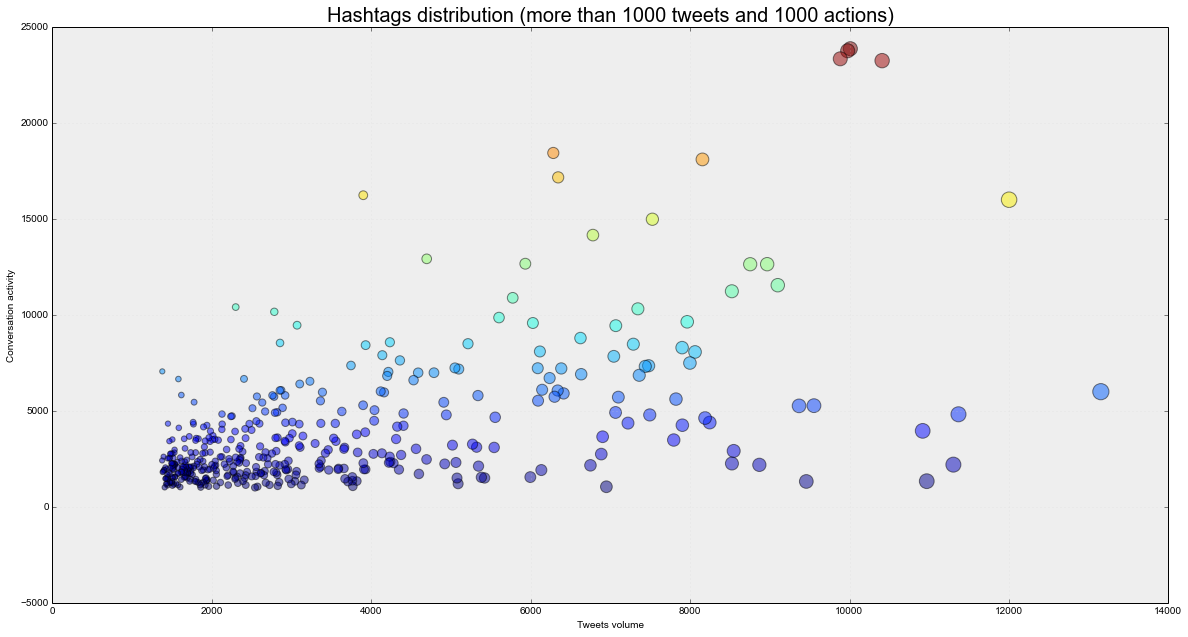
\includegraphics[width=6.0114in,height=3.2114in]{figures/chap3/chapitre3-img8.png}
    \caption{Distribution des 429 hashtags s\'electionn\'es }
\end{figure}


En proc\'edant \`a l{\textquoteright}\'etiquetage des hashtags les plus
actifs durant l{\textquoteright}ann\'ee 2012 sur Sina Weibo (figure 2
ci-dessus), nous constatons que la plupart sont associ\'es \`a des
activit\'es commerciales, de loisirs ou de divertissement. Ici nous
observons que les usages majoritaires du r\'eseau social Sina Weibo
correspondent pour la plupart \`a ceux d{\textquoteright}autres
mass-m\'edias plus traditionnels de par le monde. Le commerce en ligne
occupe notamment une place pro\'eminente. La marque de t\'el\'ephonie
mobile chinoise \textit{Xiaomi }est abondamment cit\'ee, refl\'etant
son importance croissante dans le march\'e chinois et surtout sa
strat\'egie commerciale qui cible abondamment les r\'eseaux sociaux
avec de nombreux hashtags tr\`es discut\'es (notamment
\textit{{\textquotedblleft}Fans de Xiaomi{\textquotedblright}
}[5C0F?][7C73?][7C89?][4E1D?] ). Egalement, de nombreuses campagnes
promotionnelles d{\textquoteright}ouverture ou
d{\textquoteright}anniversaire de magasins ont r\'eussi \`a se hisser
dans le jeu de t\^ete des hashtags les plus discut\'es. Radio-crochets
ou chanteurs reconnus, les stars de la t\'el\'evision et de la chanson
sont aussi pr\'esents dans le peloton de t\^etes des discussions sur
Sina Weibo. Le c\'el\`ebre chanteur Han Geng notamment compte pr\`es
d{\textquoteright}une dizaine de hashtags le concernant parmi les 500
les plus discut\'es (\textit{{\textquotedblleft}Han Geng fait une pub
pour Nokia{\textquotedblright}, {\textquotedblleft}Han Geng va en
Italie{\textquotedblright}, {\textquotedblleft}Han Geng fait une pub
Pepsi{\textquotedblright}, {\textquotedblleft}Han Geng refuse une
interview{\textquotedblright}, etc.)} Ici encore, le r\'eseau social
agit comme le prolongement des mass m\'edia traditionnels,
\'el\'ement-cl\'e des nouvelles strat\'egies de publicit\'es en ligne,
parfois particuli\`erement agressives comme dans le cas de Han Geng.
Les contenus de la t\'el\'evision sont largement relay\'es et
discut\'es, notamment les s\'eries t\'el\'evisuelles. Le cin\'ema est
aussi repr\'esent\'e. Le film comique chinois \textit{Lost in Thailand
}sorti en D\'ecembre 2012 d\'epeint les aventures d{\textquoteright}un
chinois en vacances en Thailande. Premier grand succ\`es commercial du
box-office chinois, sa popularit\'e se refl\`ete dans
l{\textquoteright}importance au sein des discussions en ligne. Les
tendances des ventes du livre sont refl\'et\'ees par de nombreux
best-seller sur {\textquotedblleft}l{\textquoteright}am\'elioration de
soi{\textquotedblright} ou la {\textquotedblleft}r\'eussite
\'economique{\textquotedblright}\textit{. }Ce type de hashtags ne se
limite pas au support web mais s{\textquoteright}origine directement
dans d{\textquoteright}autres m\'edias plus traditionnels. Le
gouvernement lui-m\^eme utilise Sina Weibo pour faire passer ses
messages avec un hashtag \textit{{\textquotedblleft}information
officielle{\textquotedblright} }utilis\'e notamment pour des d\'ementis
publics ou droit de r\'eponse par l{\textquoteright}entreprise Sina,
propri\'etaire du service. \'Egalement outil de conversation, les
discussions sur les r\'eseaux sociaux parlent de la vie de tous les
jours. La situation routi\`ere et les bouchons dans chaque ville sont
un des grands sujets de discussions. Ce sont dans ces \'echanges
quotidiens que se cristallisent plus particuli\`erement les enjeux
politiques et m\'ediatiques des r\'eseaux sociaux. Nouveau caf\'e du
commerce, les commentaires sur les faits divers et
l{\textquoteright}actualit\'e mettent souvent \`a jour les
dysfonctionnements de syst\`emes politiques, urbains ou l\'egaux. Il
est int\'eressant n\'eanmoins de noter que parmi les hashtags les plus
discut\'es, les ph\'enom\`enes de suppression de contenus par les
administrateurs (censure) restent tr\`es marginal. Le \textit{China
Digital Times} de UC Berkeley maintient une liste des mots interdits
sur Sina Weibo depuis plusieurs anne\'es \cite{Ng2013}. En comparant cette
liste de mots censur\'es \`a celle des hashtags, nous avons pu voir
qu{\textquoteright}aucun des 3000 hashtags les plus utilis\'es en 2012
n{\textquoteright}a \'et\'e soumis a une interdiction m\^eme temporaire
sur Sina Weibo. Les hashtags les plus sujets \`a la censure ne sont pas
en lien avec des domaines politiques ou des sujets sensibles, mais
plut\^ot avec des contenus \`a caract\`ere pornographique (la
pornographie est interdite en Chine). Refl\'etant les usages
majoritaires (commerce, loisirs, etc.), les hashtags v\'ehiculent des
contenus souvent moins controvers\'es et les {\textquotedblleft}mots
censur\'es{\textquotedblright} sont plus \`a m\^eme
d{\textquoteright}appara\^itre dans des discussions informelles.

\subsection[Visualisation du graphe conversationnel d{\textquoteright}utilisateurs]{Visualisation du graphe conversationnel d{\textquoteright}utilisateurs}
Apr\`es avoir identifi\'e diff\'erents \textit{m\`emes parmi }les
hashtags les plus discut\'es de l{\textquoteright}ann\'ee 2012, nous
allons maintenant proc\'eder \`a l{\textquoteright}analyse du
d\'eroulement des \'echanges d{\textquoteright}apr\`es chacun des
diff\'erents corpus de donn\'ees. Plusieurs types de graphes peuvent
\^etre extraits :


\begin{itemize}
\item \textbf{Graphe social statique : }repr\'esentant les relations
pr\'e-existantes dans la structure du r\'eseau \'etudi\'e (untel est
ami avec untel, untel suit untel, etc.)
\item \textbf{Graphe conversationnel~}: repr\'esentant toutes les
interactions qui entourent et structurent la diffusion de messages 
\item \textbf{Graphe de diffusion~}: repr\'esentant les interactions qui
se sont produites entre les acteurs durant \ la diffusion du message.
Ce dernier type de graphe est un recoupement des deux autres.
\end{itemize}


\begin{figure}
    \centering
  [Warning: Image ignored] % Unhandled or unsupported graphics:
    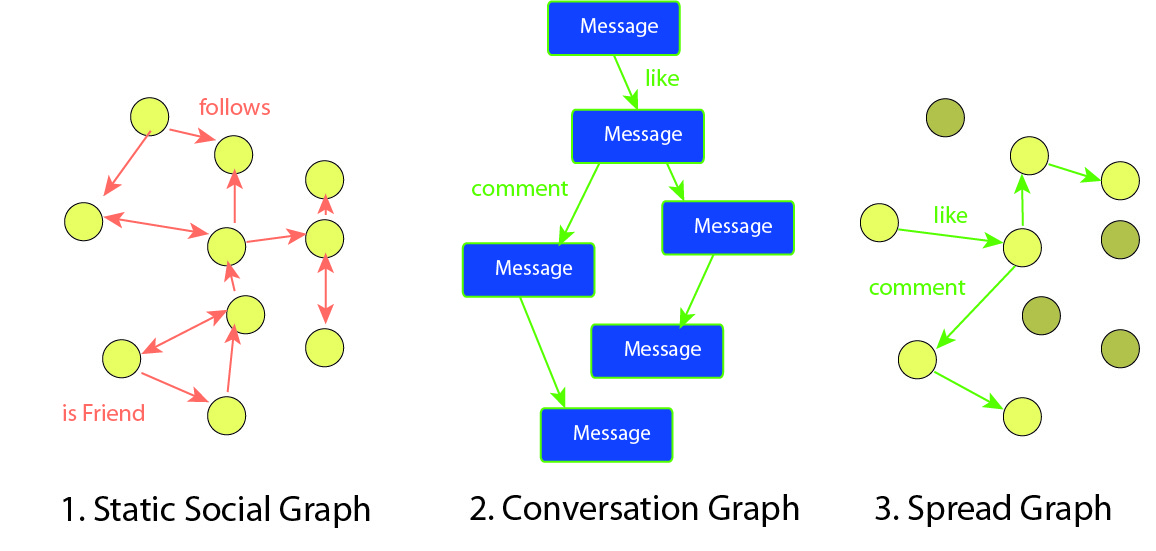
\includegraphics[width=6.2894in,height=3.0004in]{figures/chap3/chapitre3-img9.jpg}
    \caption[3 modèles de réseau]{Les 3 types de graphe classiquement extraits des donn\'ees de r\'eseaux sociaux}
\end{figure}



Dans notre \'etude, le graphe social statique ne pr\'esente pas
particuli\`erement d{\textquoteright}int\'er\^et
puisqu{\textquoteright}il correspond \`a un ensemble de relations peu
affect\'e par les discussions. De plus, nous ne disposons dans le jeu
de donn\'ees Weiboscope que de son \'etat final qui ne t\'emoigne pas
de l{\textquoteright}\'evolution des relations. Nous voulons obtenir
ici les graphes de diffusion sous la forme de conversations
structur\'ees\textbf{~(}graphe directionnelle des \ r\'eponses et
commentaires) de l{\textquoteright}ensemble des messages. Dans un
article paru dans \textit{Nature} \cite{Weng2012}, les chercheurs du
\textit{Centre de Recherche sur les Syst\`emes Complexes} de
l{\textquoteright}Universit\'e d{\textquoteright}Indiana identifient
les caract\'eristiques des m\`emes connaissant le plus de succ\`es (la
plus large diffusion). Un travail de visualisation de m\`emes
identifi\'es par des hashtags sur Twitter leur permet notamment de
mettre \`a jour des motifs particuliers dans la structure des
conversations.



\begin{figure}
    \centering
    \centering
    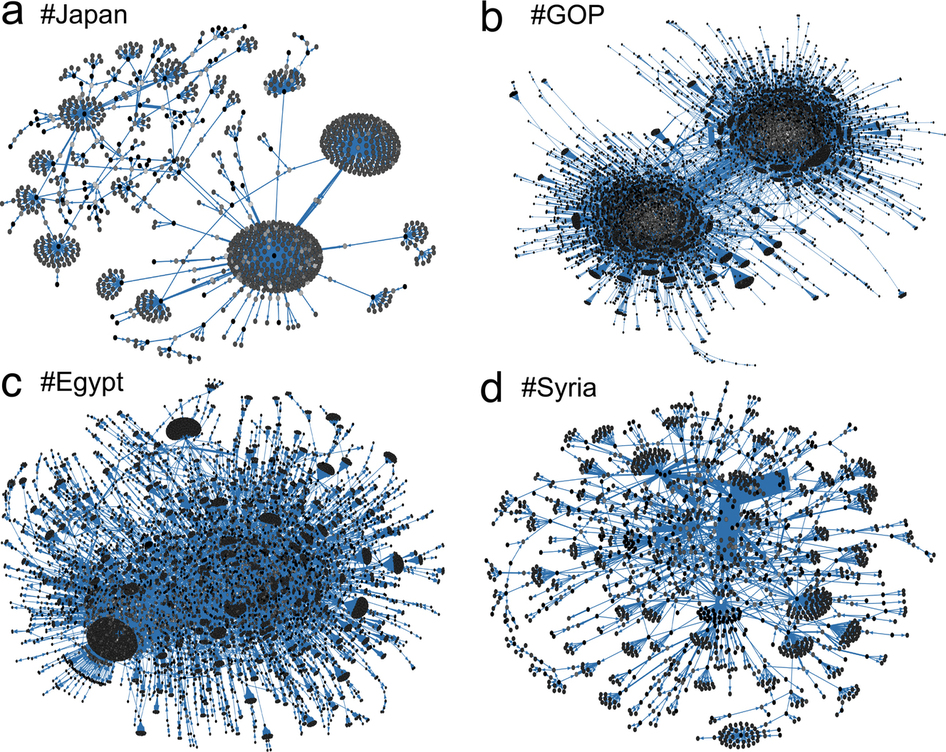
\includegraphics[width=5.5669in,height=4.4224in]{figures/chap3/chapitre3-img10.jpg}

    Nodes represent Twitter users, and directed edges represent retweeted posts that carry the meme. The brightness of a node indicates the activity (number of retweets) of a user, and the weight of an edge reflects the number of retweets between two users. \newline
    (a) The \textit{\#Japan}  meme shows how news about the March 2011 earthquake propagated. \newline
    (b) The \textit{\#GOP} tag stands for the US Republican Party and as many political memes, displays a strong polarization between people with opposing views. \newline
    Memes related to the Arab Spring and in particular the 2011 uprisings in (c) \textit{\#Egypt} and (d) \textit{\#Syria} display characteristic hub users and strong connections, respectively.
    
    \caption{Graphe de diffusion de hashtags sur Twitter d{\textquoteright}apr\`es \cite{Weng2012} }

\end{figure}


Afin de mettre \`a jour le graphe conversationnel entourant les hashtags
s\'electionn\'es sur Sina Weibo, nous avons choisi
d{\textquoteright}extraire la s\'equence d{\textquoteright}interactions
des messages (mentions, retweets) composant chaque m\`eme. Cette
structure de graphe nous permet de repr\'esenter la diffusion de chaque
m\`eme sous forme d{\textquoteright}un graphe contenant un node par
utilisateur et un ensemble de relations correspondant aux \'echanges
visibles dans les textes des messages. Dans un premier temps, le
logiciel \textit{Graphviz }nous a permis d{\textquoteright}obtenir une
repr\'esentation basique du graphe conversationnel afin
d{\textquoteright}avoir un aper\c{c}u sur la nature des conversations
par l{\textquoteright}observation des motifs qui la compose. En effet,
si les deux mesures identifi\'ees \`a l{\textquoteright}\'etape
pr\'ec\'edente (volume de messages et \ volume
d{\textquoteright}\'echanges) nous permettent
d{\textquoteright}effectuer un premier tri parmi les hashtags, cette
premi\`ere visualisation nous permet de consid\'erer la nature des
\'echanges et l{\textquoteright}implication des utilisateurs
d{\textquoteright}apr\`es la structure des motifs conversationnels.
Chaque utilisateur est symbolis\'e par un point et chaque message par
un trait reliant deux utilisateurs. Un motif tr\`es compact refl\`ete
une conversation anim\'ee entre des utilisateurs peu nombreux
\'echangeant beaucoup. A l{\textquoteright}inverse, un motif disparate
refl\`ete des \'echanges plus brefs et morcel\'es.

\begin{figure}
    \centering
    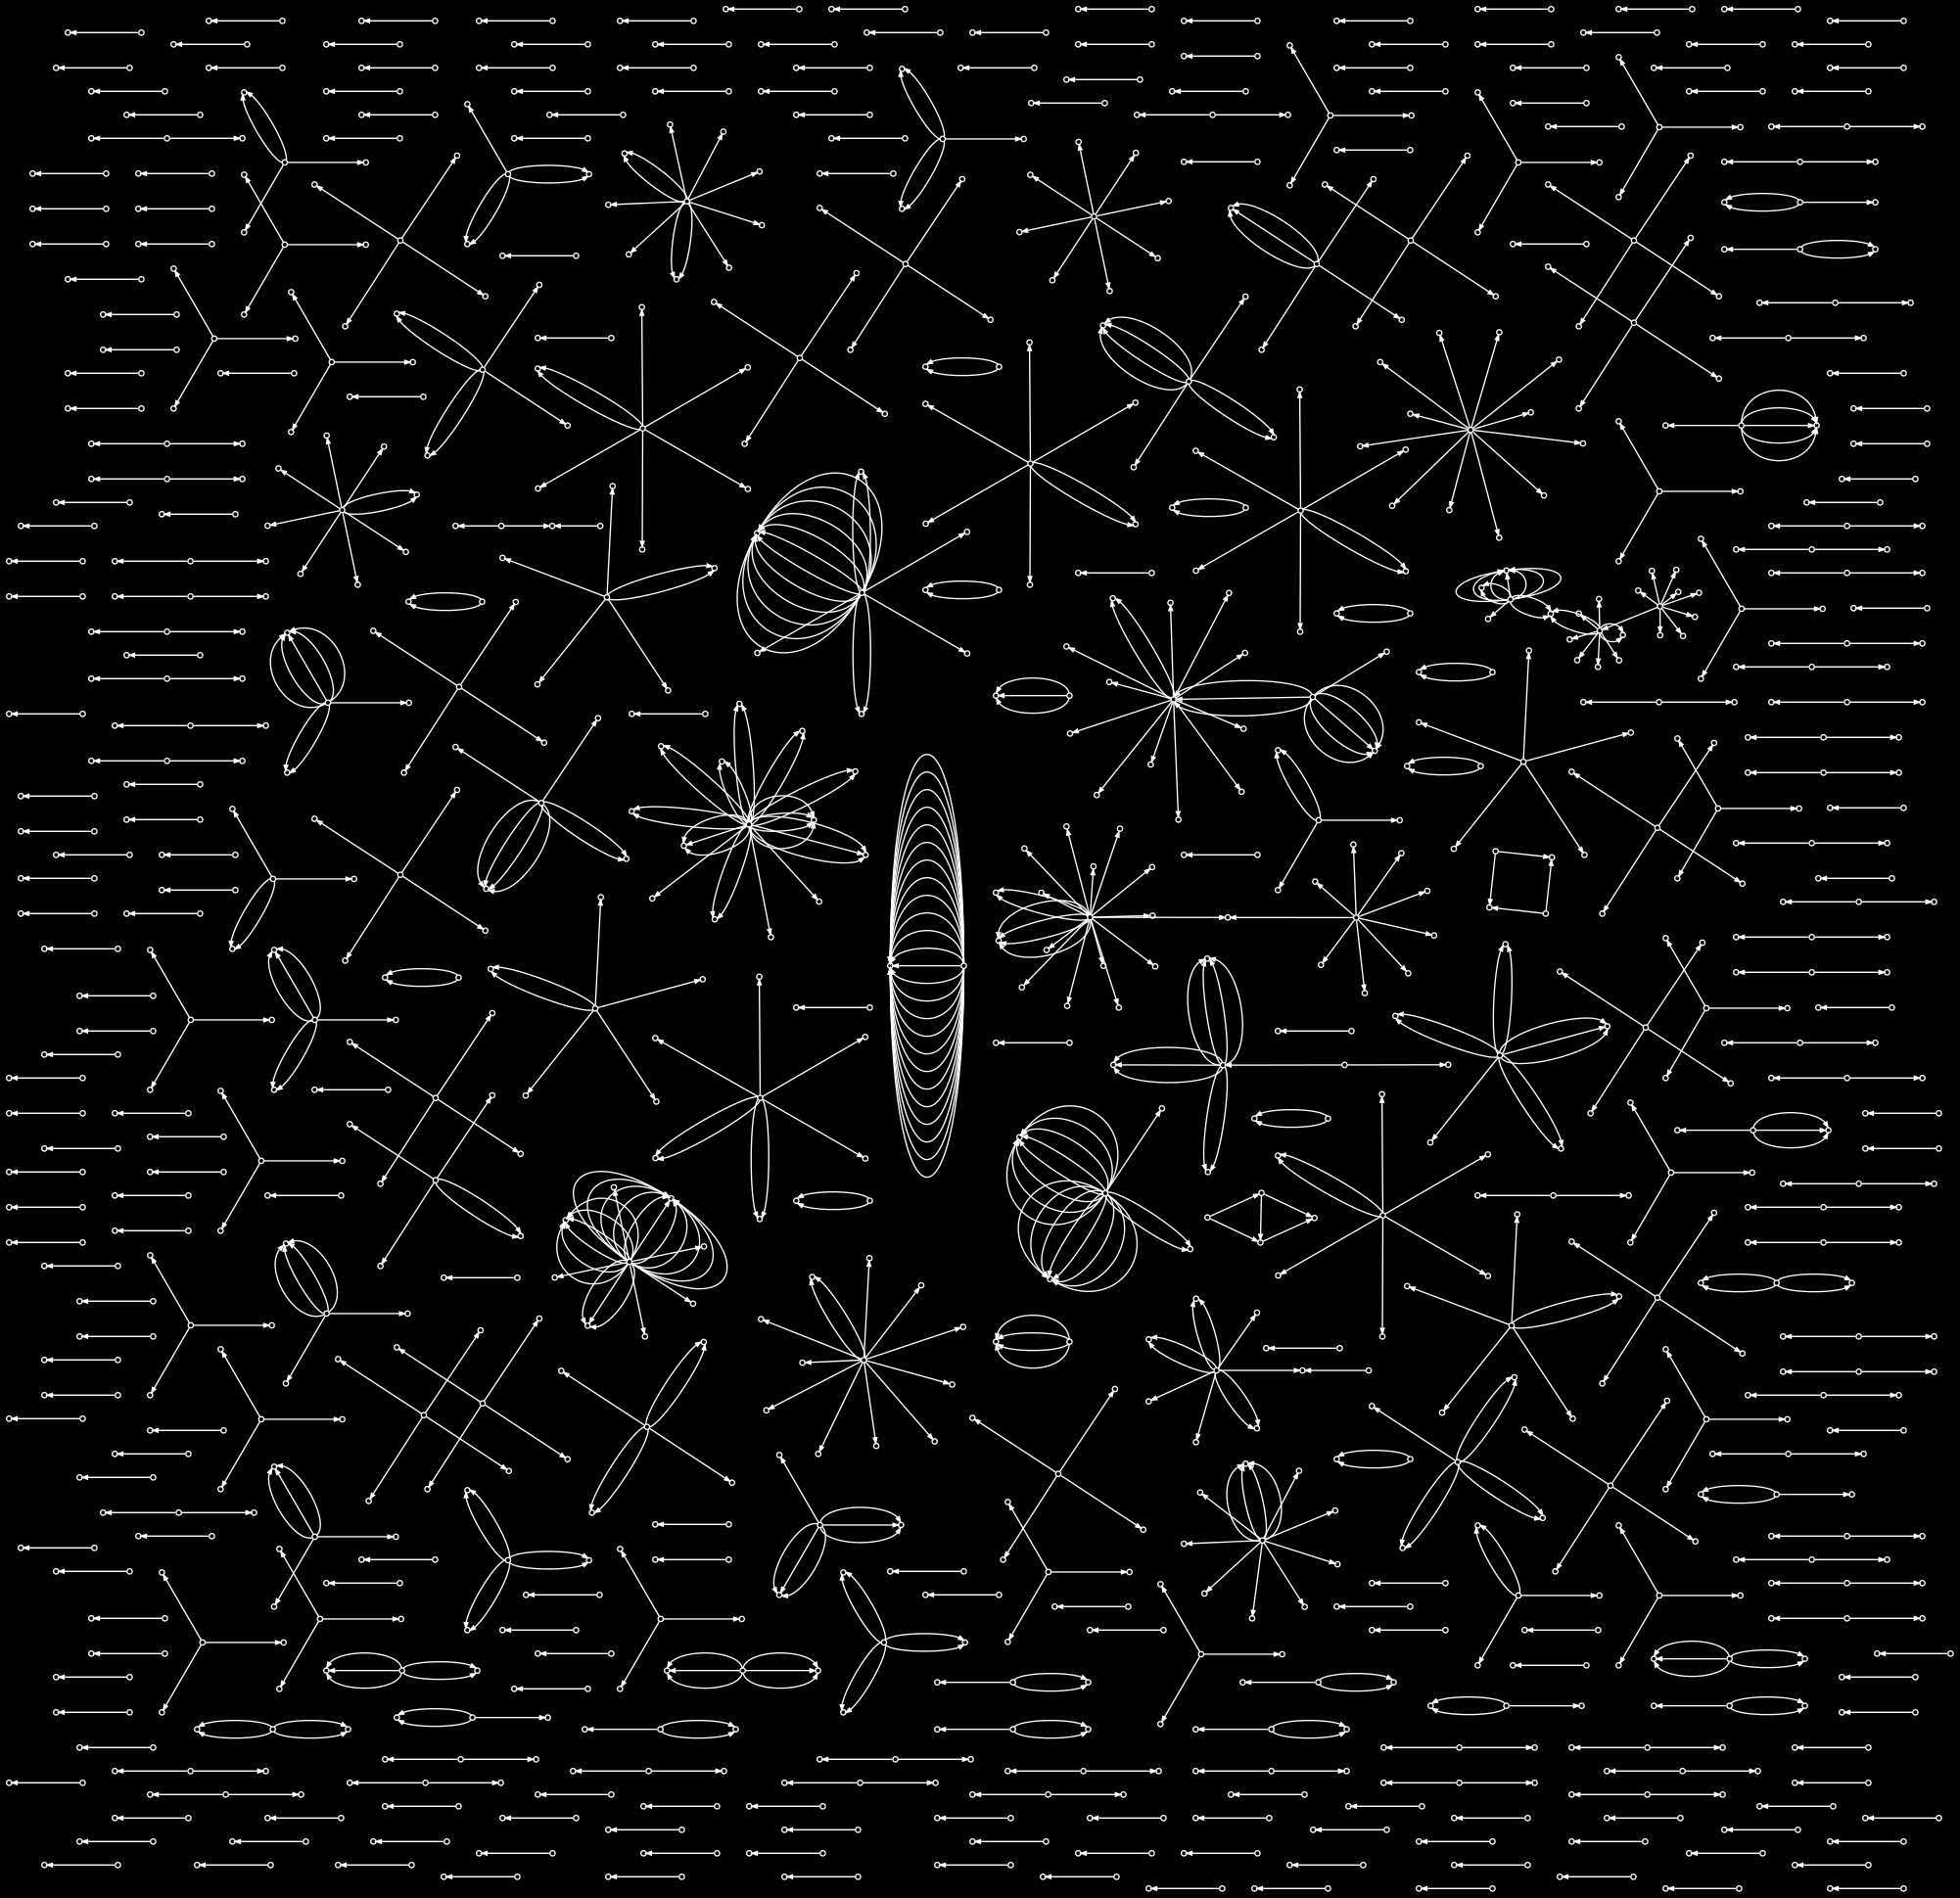
\includegraphics[width=5.5894in,height=5.4224in]{figures/chap3/chapitre3-img11.png}
    \caption[Visualisation simple du hashtag{\textquotedblleft}WeicoPlus{\textquotedblright}] {Fig. Visualisation simple du hashtag{\textquotedblleft}WeicoPlus{\textquotedblright}, un trait repr\'esente un \'echange entre deux utilisateurs}
\end{figure}

\textit{WeicoPlus }est une application mobile permettant
d{\textquoteright}utiliser Sina Weibo. Le hashtag \#WeicoPlus\# est
ajout\'e automatiquement quand les utilisateurs postent des photos
depuis ce service. Ainsi, on remarque que le graphe conversationnel
entourant WeicoPlus se compose essentiellement de messages simples,
mais ne donne pas lieu \`a une conversation structur\'ee - \`a
l{\textquoteright}exception de quelques rapides \'echanges entre un
nombre r\'eduit de personnes.



\begin{figure}
    \centering
    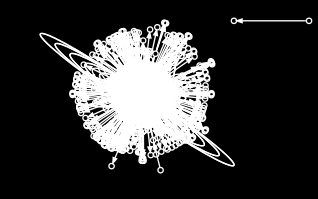
\includegraphics[width=5.0449in,height=3.1559in]{figures/chap3/chapitre3-img12.png}
    \caption[Visualisation simple des conversations autour du hashtag Veuve d{\textquoteright}enfant unique]{Visualisation simple des conversations autour du hashtag Veuve d{\textquoteright}enfant unique}
\end{figure}

A l{\textquoteright}inverse, le hashtag {\textquotedblleft}Veuve
d{\textquoteright}enfant
unique{\textquotedblright}[FF08?]\#[5931?][72EC?][6BCD?][4EB2?]\#[FF09?]cristallise
le d\'ebat en une forme tr\`es dense qui refl\`ete une surench\`ere de
commentaires et d{\textquoteright}actions autour du hashtag, propre
d{\textquoteright}une conversation anim\'ee. 

\subsection[Premiers \'el\'ements d{\textquoteright}analyse: visualisation de m\`emes ]{Premiers \'el\'ements d{\textquoteright}analyse: visualisation de m\`emes }
Les diff\'erents mod\`eles de conversation que nous obtenons dans cette
premi\`ere \'etape se pr\'esentent sous une forme sch\'ematique et peu
d\'etaill\'ee. Afin de comprendre plus en d\'etails les dynamiques
conversationnelles qui les entourent, nous avons choisi de
s\'electionner trois exemples parlants de hashtags dont les graphes
conversationnels pr\'esentent des particularit\'es des mod\`eles de
diffusion dissemblables et organis\'es. Pour chacun
d{\textquoteright}eux, nous allons proc\'eder \`a une analyse plus
d\'etaill\'ee des graphes conversationnels afin de consid\'erer les
diff\'erences entre ces diff\'erents mod\`eles.



\begin{figure}
    \centering
\centering
    \subfloat[Pluie torrentielle \`a Tianjing]{
        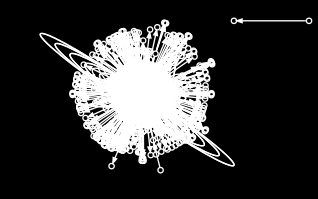
\includegraphics[width=2.3224in,height=1.4449in]{figures/chap3/chapitre3-img13.png}
    }

    \subfloat[Veuve \`a l{\textquoteright}enfant unique]{
        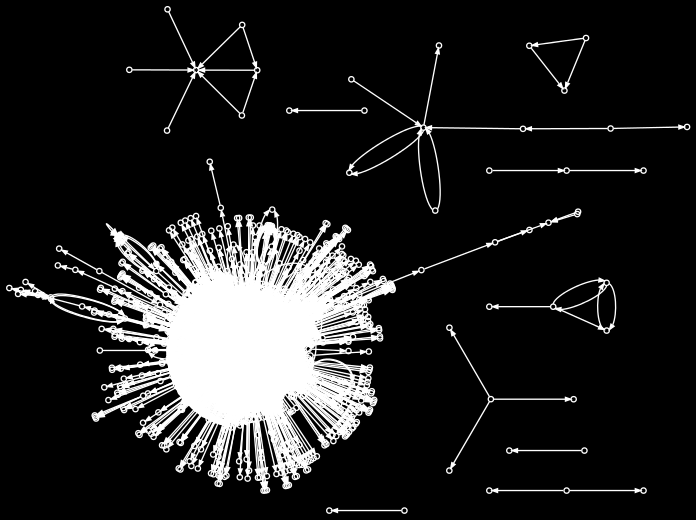
\includegraphics[width=2.3004in,height=1.7224in]{figures/chap3/chapitre3-img14.png}
    }


    \subfloat[Abolition des lois sur la prostitution]{
        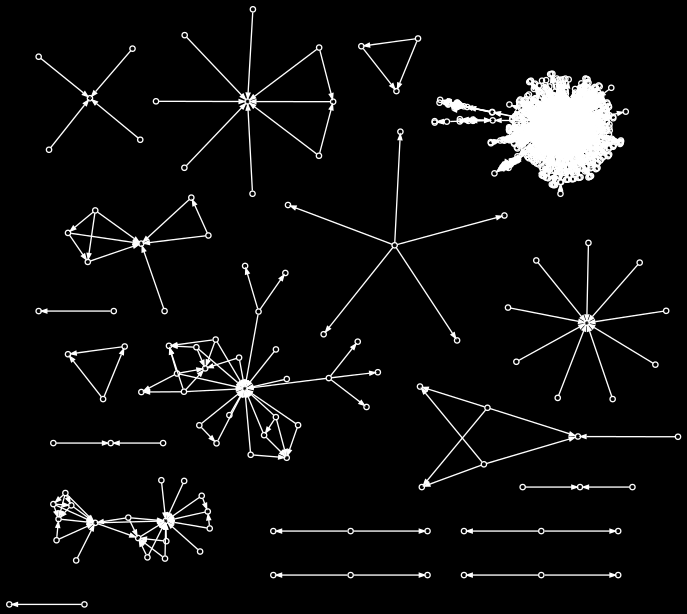
\includegraphics[width=2.1449in,height=1.9224in]{figures/chap3/chapitre3-img15.png}   
    }
  
    \caption{Visualisation des réseaux de conversation}
\end{figure}


Nous voyons que les trois repr\'esentations des graphes ci-dessus
donnent \`a voir des structures plus ou moins morcel\'ees, avec un
ensemble de points et de lignes tr\`es compactes qui repr\'esentent la
majeure partie de la conversation. Afin de visualiser plus
pr\'ecis\'ement les groupes et les dynamiques qui constituent les
discussions autour de chaque hashtag, nous allons utiliser le logiciel
Gephi \cite{Bastian2013} afin d{\textquoteright}examiner de plus pr\`es la
composition de ces graphes. Pour ce faire, Gephi va nous permettre
d{\textquoteright} {\textquotedblleft}\'etaler{\textquotedblright} le
graphe en repositionnant les nodes et en les coloriant pour en
identifier les composantes et les tendances.

Chaque utilisateur est repr\'esent\'e sous la forme d{\textquoteright}un
point. La taille des points correspond \`a l{\textquoteright}importance
de l{\textquoteright}utilisateur dans le r\'eseau tot\ \ al des
\'echanges, caract\'eris\'e par son degr\'e de centralit\'e
interm\'ediaire (\textit{betweenness centrality}), une mesure
topologique correspondant au nombre de plus courts chemins du graphe
passant par cet utilisateur. La couleur est utilis\'ee pour
repr\'esenter la \textit{modularit\'e }du r\'eseau,
c{\textquoteright}est \`a dire le nombre de communaut\'es engag\'ees
dans la conversation d\'efinies comme les cliques
d{\textquoteright}utilisateurs constituant plus de 1\% du r\'eseau
total d{\textquoteright}\'echange \cite{Blondel2008}. La position
des nodes est calcul\'ee gr\^ace \`a l{\textquoteright}algorithme
\textit{Force Atlas 2} \cite{Jacomy2012} utilisant une
mod\'elisation physique o\`u les nodes peu connect\'es entre eux se
repoussent et ceux tr\`es connect\'es s{\textquoteright}attirent.
Ainsi, la proximit\'e de deux nodes sur le graphe t\'emoigne
d{\textquoteright}une proximit\'e lors des conversations,
c{\textquoteright}est \`a dire de l{\textquoteright}existence
d{\textquoteright}un \'echange entre eux (citations, commentaires ou
retweets). Pour davantage de visibilit\'e, certaines conversations
sub-alternes repr\'esentant moins de 1\% du total ont \'et\'e
effac\'ees. Egalement, les nodes poss\'edant un degr\'e inf\'erieur \`a
3 (moins d{\textquoteright}un \'echange avec au moins trois autres
nodes du grahe) ne sont pas repr\'esent\'ees.



\textbf{Exemple 1 : Pluie torrentielle \`a Tianjing}

Le premier m\`eme choisi parle d{\textquoteright}une catastrophe
naturelle, sous la forme d{\textquoteright}une pluie diluvienne qui
s{\textquoteright}est abattue sur la ville de Tianjin durant la nuit du
21 au 22 Juillet 2012. 

\begin{figure}
    \centering
    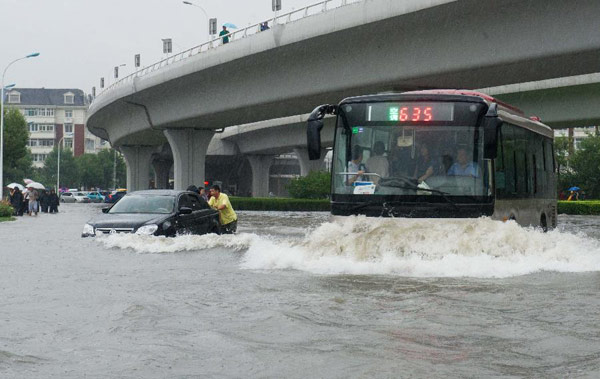
\includegraphics[width=6.0114in,height=3.7894in]{figures/chap3/chapitre3-img16.jpg}
    \caption[Photo de Tianjin durant la pluie torentielle en Juillet 2012]{\textit{Downpour bypasses Beijing, batters neighbor, }in Qinghua News le 2012-07-26 13:29:59, \url{http://news.xinhuanet.com/english/china/2012-07/26/c_131740415.htm} consult\'e le 27 Juin 2014.}
\end{figure}

Ici 4 groupes composent 85\% du graphe, constitu\'es autour de gros
diffuseurs (les nodes les plus gros). Plusieurs groupes semblent
s{\textquoteright}emparer de la conversation mais on voit peu
d{\textquoteright}activit\'e entre les nodes alors que les \'echanges
se d\'eroulent autour de quelques utilisateurs tr\`es centraux. Cela
traduit le fait que peu de personnes ont r\'eellement discut\'e
l{\textquoteright}information et elles se sont simplement content\'es
de la relayer.


\begin{figure}
    \centering
    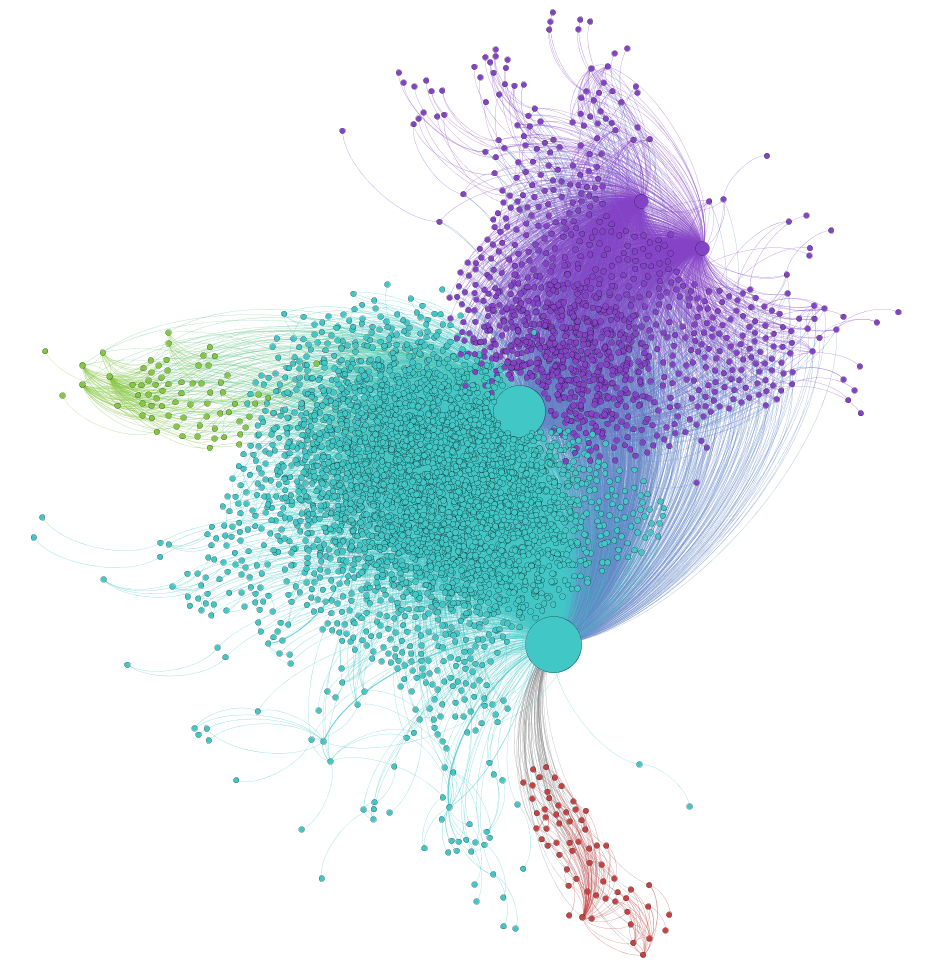
\includegraphics[width=6.0114in,height=6.0114in]{figures/chap3/chapitre3-img17.png}
    \caption{Exemple 1 : Tianjin Baoyu}
\end{figure}

La diffusion d{\textquoteright}un fait divers tr\`es local (il se passe
\`a Tianjing) est entrain\'ee par peu de sources tr\`es importantes
(les quelques nodes de grande taille), vraisemblablement des journaux
et m\'edias locaux qui annoncent la nouvelle (presse, photos-choc
d{\textquoteright}innondations, etc). La conversation est peu active et
tr\`es structur\'ee, nous sommes en pr\'esence d{\textquoteright}un
mod\`ele classique de diffusion de masse.

\textbf{Exemple 2 : Veuve de l{\textquoteright}enfant unique}

Un autre sujet discut\'e par une tr\`es large quantit\'e de personnes
appara\^it sous le terme {\textquotedbl}\textit{shidu
muqin}{\textquotedbl}, forme contract\'ee signifiant
\textit{{\textquotedblleft}m\`ere qui a perdu son enfant
unique{\textquotedblright}
(}[5931?][53BB?][72EC?][751F?][5B50?][5973?][7684?][6BCD?][4EB2?]). Ce
hashtag d\'esigne un ph\'enom\`ene de soci\'et\'e bien connu en Chine
o\`u le deuil de la perte d{\textquoteright}un enfant se double souvent
pour une m\`ere chinoise seule de l{\textquoteright}absence de
ressources pour vivre. En effet, l{\textquoteright}absence de syst\`eme
de retraite fait porter aux enfants la responsabilit\'e de la survie de
la famille. 

Le graphe ici est fait de deux grands groupes composant \`a eux deux
pr\`es de 95\% du graphe total. Les discussions sont tr\`es
polaris\'ees et men\'ees par peu de participants (les nodes les plus
gros sur le graphe). Peu de personnes tr\`es influentes concentrent les
discussions autour d{\textquoteright}eux, accompagn\'es ou suivis
d{\textquoteright}une foule de commentateurs. 

\begin{figure}
    \centering
    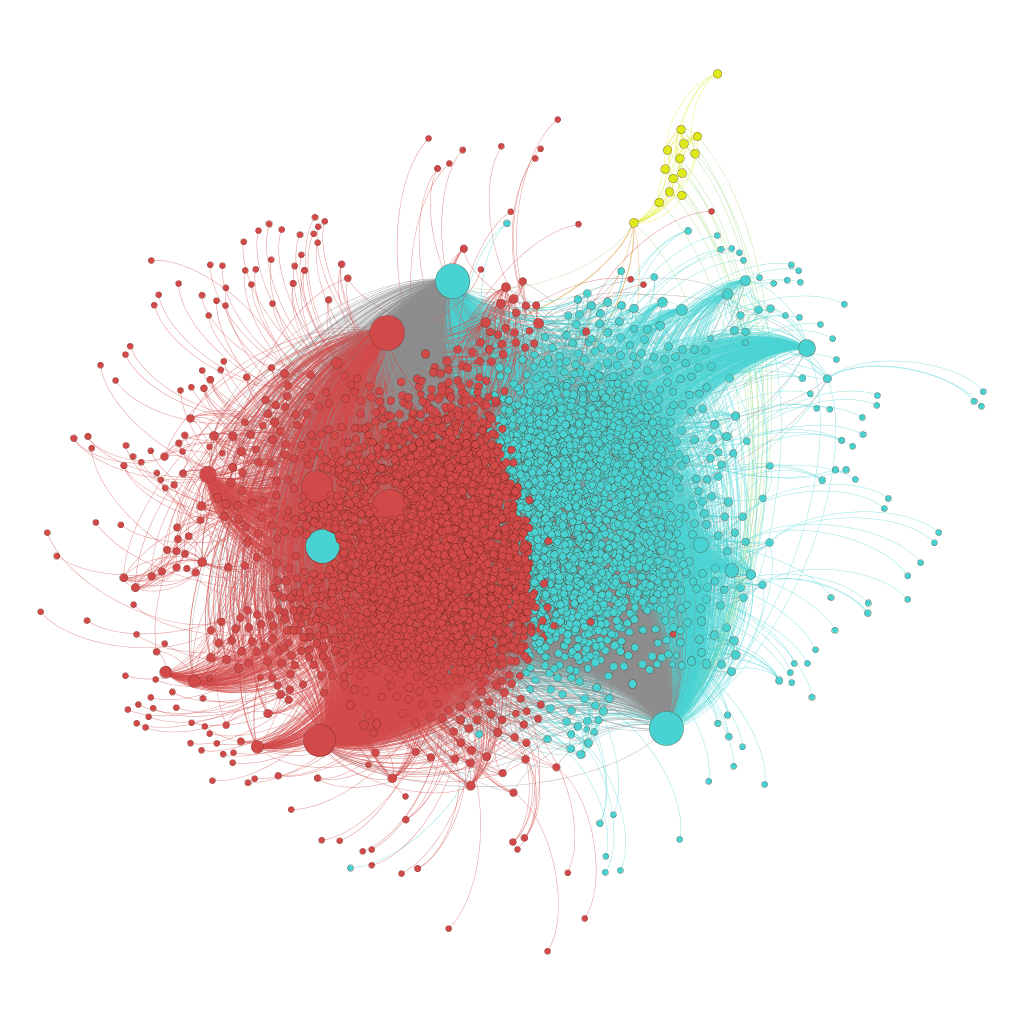
\includegraphics[width=6.0114in,height=6.0114in]{figures/chap3/chapitre3-img18.png}
    \caption{{\textquotedblleft}Shidu Muqin{\textquotedblright}}
\end{figure}


Cet exemple donne \`a voir des groupes bien d\'efinis et tr\`es proches
o\`u plusieurs acteurs majeurs m\`enent la discussion. Les dynamiques
d{\textquoteright}\'echanges autour d{\textquoteright}une question de
soci\'et\'e (la loi de l{\textquoteright}enfant unique en Chine et ses
cons\'equences) s{\textquoteright}articule en groupes distincts sans
pour autant amener \`a des controverses importantes (qui se
traduiraient par des discussions longues et houleuses). Ici, les
leaders d{\textquoteright}opinion font la discussion et la diffusion se
fait au travers d{\textquoteright}eux.

\clearpage
\textbf{Exemple 3 : Abolition des lois sur la prostitution}

Le hashtag \textit{{\textquotedblleft}Abolissons la loi piaowudong
nuzui{\textquotedblright} }est l{\textquoteright}expression
d{\textquoteright}une campagne pour l{\textquoteright}abolition
d{\textquoteright}une l\'egislation scandaleuse sur la prostitution en
Chine. Depuis les ann\'ees 80, la loi chinoise interdit la prostitution
et pr\'evoit la condamnation des deux parties qui
s{\textquoteright}adonnent \`a un \'echange d{\textquoteright}argent.
Baptis\'e \textit{{\textquotedblleft}Piaowudong
nuzui{\textquotedblright}, }cette loi a vu plusieurs cas absurdes
impliquant des viols organis\'es sur mineurs se solder par la
condamnation et l{\textquoteright}emprisonnement des enfants
incrimin\'es. Relay\'es par les journalistes, les scandales \`a
r\'ep\'etition ont \'eclat\'es \`a plusieurs reprises, impliquant
parfois des officiels du Parti souvent blanchis alors que des enfants
\'etaient eux emprisonn\'es. Le graphe des discussions autour de
l{\textquoteright}abolition de cette loi montre que de nombreux groupes
discutent s\'epar\'ement de cette question puisque les premiers 50\% du
graphe sont d\'ej\`a constitu\'es de plus d{\textquoteright}une
quinzaine de clusters. Les groupes sont tr\`es \'eloign\'es entre eux,
n{\textquoteright}entretenant que peu de relations et connaissant une
activit\'e intense.

\begin{figure}
    \centering
    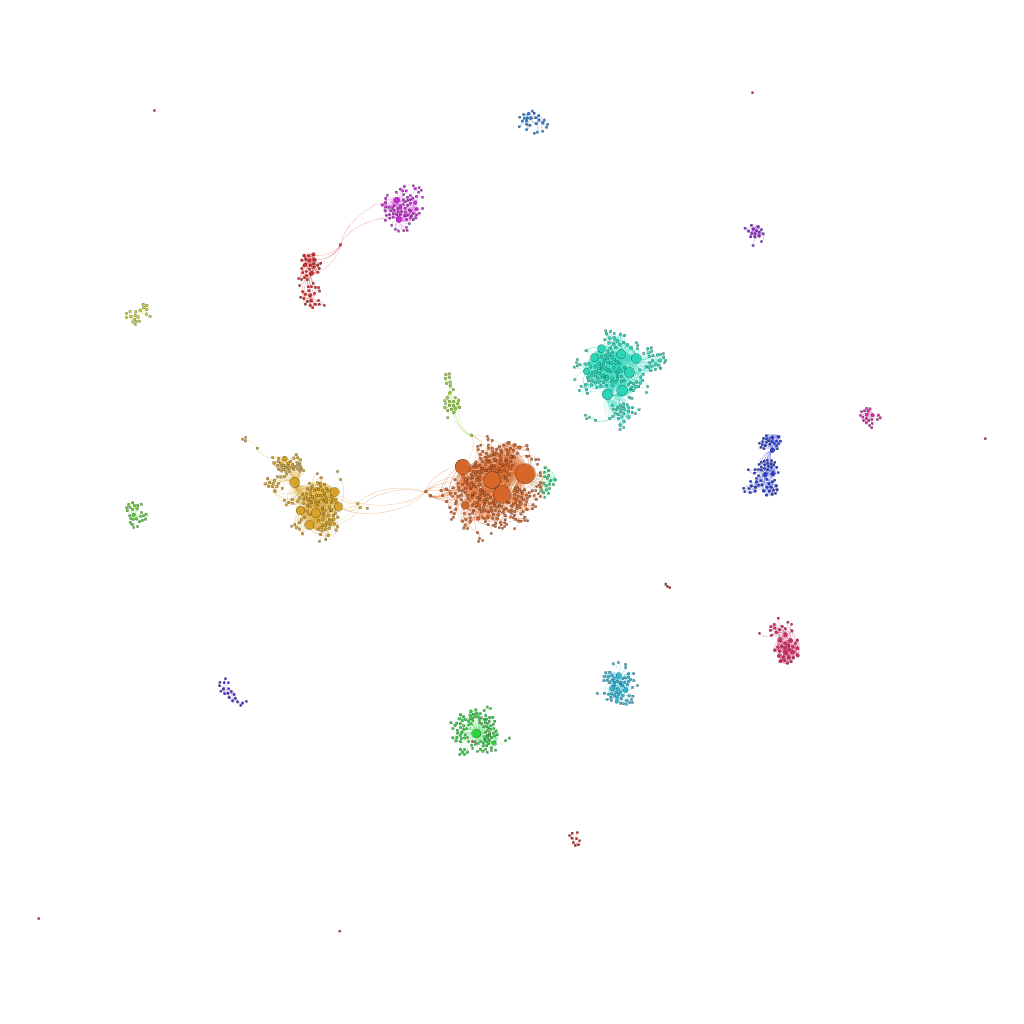
\includegraphics[width=6.0114in,height=6.0114in]{figures/chap3/chapitre3-img19.png}
    \caption{ {\textquotedblleft}Piaowudong nuzui{\textquotedblright}}
\end{figure}

Cet exemple pr\'esente les caract\'eristiques d{\textquoteright}une
conversation tr\`es d\'ecentralis\'ee dans laquelle de nombreux acteurs
diff\'erents prennent part. L{\textquoteright}\'emergence de ce type de
discussion fragment\'ee t\'emoigne d{\textquoteright}un usage
particulier de la discussion sur le r\'eseau social et montre comment
la discussion autour d{\textquoteright}un sujet peut
s{\textquoteright}\'etendre sans afficher de relations directes dans le
m\'edia lui-m\^eme. Ici un agent ext\'erieur (en
l{\textquoteright}occurence un article du journal \textit{Nanfang
Zhoumo }sur le sujet) fait na\^itre la conversation sans pour autant
l{\textquoteright}accaparer et la centraliser. Plus difficilement
d\'etectable et contr\^olable, cette derni\`ere configuration est
typique du m\`eme car elle se d\'eveloppe de fa\c{c}on large et durable
entre des groupes \`a l{\textquoteright}origine peu connect\'es.

Cette premi\`ere visualisation des graphes conversationnels nous permet
d{\textquoteright}explorer quelques types pr\'ecis
d{\textquoteright}\'echanges et d{\textquoteright}en proposer une
premi\`ere lecture. N\'eanmoins, le proc\'ed\'e de visualisation reste
rudimentaire et soul\`eve plusieurs questions que nous nous donnons
pour t\^ache de continuer \`a explorer. Premi\`erement, dans quel
espace a lieu cette repr\'esentation? En \'etalant ainsi ces graphes
conversationnels, quelle action r\'ealisons-nous r\'eellement et quelle
en est la valeur pour l{\textquoteright}analyse? \`A plus forte raison,
quelle est la relation de cette espace du graphe conversationnel avec
les autres formes d{\textquoteright}espace, et plus notamment
l{\textquoteright}espace du r\'eel g\'eographique et
l{\textquoteright}espace de la repr\'esentation par le langage? 

\section{M\'ethodologie de traitement et de visualisation des m\`emes}
L{\textquoteright}\'etude des relations entre ces diff\'erents types
d{\textquoteright}espaces implique donc une m\'ethodologie renouvel\'ee
et le d\'eveloppement d{\textquoteright}outils adapt\'es. Il ne
s{\textquoteright}agit plus simplement d{\textquoteright}\'etudier un
r\'eseau, mais plus pr\'ecis\'ement de s{\textquoteright}interroger sur
les relations entre diff\'erents r\'eseaux, de nature souvent
diff\'erentes. Au-del\`a du r\'eseau multi-calques, nous sommes en
pr\'esence de multiples r\'eseaux poss\'edant des relations communes.

Nous avons donc s\'electionn\'e trois aspects importants des m\`emes que
nous allons tenter de repr\'esenter au mieux afin d{\textquoteright}en
comprendre l{\textquoteright}existence :

\textbf{{}- }\textbf{\textit{langagier }}\textbf{:} le champ
s\'emantique d{\textquoteright}un m\`eme est constitu\'e des mots qui
sont prononc\'es lors de sa diffusion. L{\textquoteright}association de
mots -souvent sous la forme du jeu de mots - est un des propres du
m\`eme et constitue ainsi une part importante de son existence. Ainsi,
le m\`eme produit \`a proprement parler des r\'eseaux de mots en
dessinant des liens entre des signifiants souvent improbables qui en
font souvent le succ\`es \cite{Bauckhage2011}.

\textbf{\textit{{}- conversationnel }}\textit{: }au-del\`a des mots, un
m\`eme se constitue sous la forme d{\textquoteright}un \'echange, une
conversation o\`u les diff\'erents acteurs discutent, commentent et se
saisissent des actions disponibles sur la pateforme web (like,
retweets, etc.) pour converser. Comme nous l{\textquoteright}avons vu
pr\'ec\'edemment, nous pouvons identifier et consid\'erer un graphe
conversationnel cr\'e\'e par le m\`eme en se diffusant.

\textbf{\textit{{}- r\'eel : }}au-del\`a des \'echanges en ligne, ces
discussions poss\`edent une existence physique, premi\`erement sous la
forme de l{\textquoteright}activit\'e \'electrique des machines qui
sont utilis\'ees lors de ce processus. N\'eanmoins, dans
l{\textquoteright}approche d{\textquoteright}une g\'eographie humaine
des \'echanges num\'eriques, nous consid\'ererons ici
l{\textquoteright}existence physique des m\`emes par celle des
utilisateurs - de leurs corps - et non pas des machines.

Afin d{\textquoteright}\'etudier chacun de ces aspects du m\`eme, nous
allons donc proc\'eder \`a la collection et la visualisation de
donn\'ees sur chacun de ces niveaux d{\textquoteright}apr\`es un corpus
de m\`emes s\'electionn\'es.

\subsection[S\'election de m\`emes pour l{\textquoteright}\'etude]{\textmd{\textup{ S\'election de
m\`emes pour l{\textquoteright}\'etude}}}
Choisir un ensemble de m\`emes coh\'erents est une des \'etapes
difficiles de notre recherche. En effet, dans le vaste corpus de
donn\'ees utilis\'ees et plus g\'en\'eralement dans la multitude des
\'echanges quotidiens sur les r\'eseaux sociaux, trouver une prise pour
l{\textquoteright}\'etude n{\textquoteright}est pas une t\^ache
\'evidente. Afin de proc\'eder \`a la s\'election de m\`emes, nous
avons donc choisi d{\textquoteright}utiliser la typologie des
cat\'egories de m\`emes identifi\'ees dans la litt\'erature (voir
partie 2) et d{\textquoteright}en syst\'ematiser
l{\textquoteright}usage sur notre corpus. Ainsi, pour chaque
cat\'egorie, nous avons effectu\'e une recherche m\^elant des sources
parlant des m\`emes et de l{\textquoteright}Internet chinois (journaux,
blogs, encyclop\'edies en ligne, sites ressources), notre propre
exp\'erience du web chinois et notre corpus de donn\'ees disponibles.

Dans un premier temps, nous avons donc identifi\'e pour chaque
cat\'egorie de m\`eme plusieurs \'ev\`enements web de
l{\textquoteright}ann\'ee 2012 sur Sina Weibo comme autant de candidats
pour repr\'esenter l{\textquoteright}ensemble de notre typologie. La
classification de l{\textquoteright}importance des \'ev\`enements web
rev\^et une nature tr\`es diff\'erente selon les diff\'erentes sources.
Une revue de la litt\'erature web sur les
{\textquotedblleft}\'ev\`enements marquant du web social en
2012{\textquotedblright} montre que les contenus \`a caract\`ere
politique et pol\'emique sont consid\'er\'es comme plus importants sur
les sites \`a audience majoritairement occidentale\footnote{ Global
Voices,
\ \ \ \url{http://globalvoicesonline.org/2012/12/07/top-10-chinese-internet-memes-of-2012/,}
consult\'e le 22 Avril 2014 \`a 12:10 ou WSJ
http://blogs.wsj.com/chinarealtime/2012/12/19/the-top-10-chinese-internet-memes-of-2012/,
consult\'e le 22 Avril 2014 \`a 12:10 } alors que les sites plus
sp\'ecialis\'es sur la Chine\footnote{ Danwei
\ \url{http://www.danwei.com/chinas-hottest-styles-of-2012/}
\ consult\'e le 22 Avril 2014 \`a 12:12} prennent davantage en
consid\'eration les ph\'enom\`enes m\'ediatiques commerciaux. Encore
une fois, nous voyons comment les r\'eseaux sociaux chinois sont
repr\'esent\'es comme des ph\'enom\`enes politiques, parfois au
d\'etriment de leur existence comme m\'edia \`a part enti\`ere. Apr\`es
avoir compar\'e ces sources diverses, il nous fallait \^etre s\^ur que
nous disposions d{\textquoteright}une quantit\'e suffisante de
donn\'ees pour traiter le m\`eme choisi. Nous avons donc index\'e les
parties du corpus repr\'esentatives des diff\'erents \'ev\`enements
afin de pouvoir effectuer des \ recherches plein-texte et ainsi
v\'erifier le volume et la qualit\'e des corpus mobilisables pour
chaque m\`eme. Pour ce faire, nous avons mis en place un outil
d{\textquoteright}indexation et de recherche\footnote{ Les technologies
utilis\'ees pour indexer le corpus sont \textit{ElasticSearch }pour le
moteur de recherche et \textit{Kibana} pour le tableau de bord.
\url{http://www.elasticsearch.org} consult\'e le 22 Avril 2014 \`a
12:23} qui nous permet de contr\^oler les diff\'erents param\`etres et
nous assurer de la quantit\'e (taille significative), des dimensions
(dates correctes) et de la qualit\'e du corpus (v\'erification du
contenu d{\textquoteright}un \'echantillon de 100 messages
s\'electionn\'es al\'eatoirement).


\begin{figure}
    \centering
    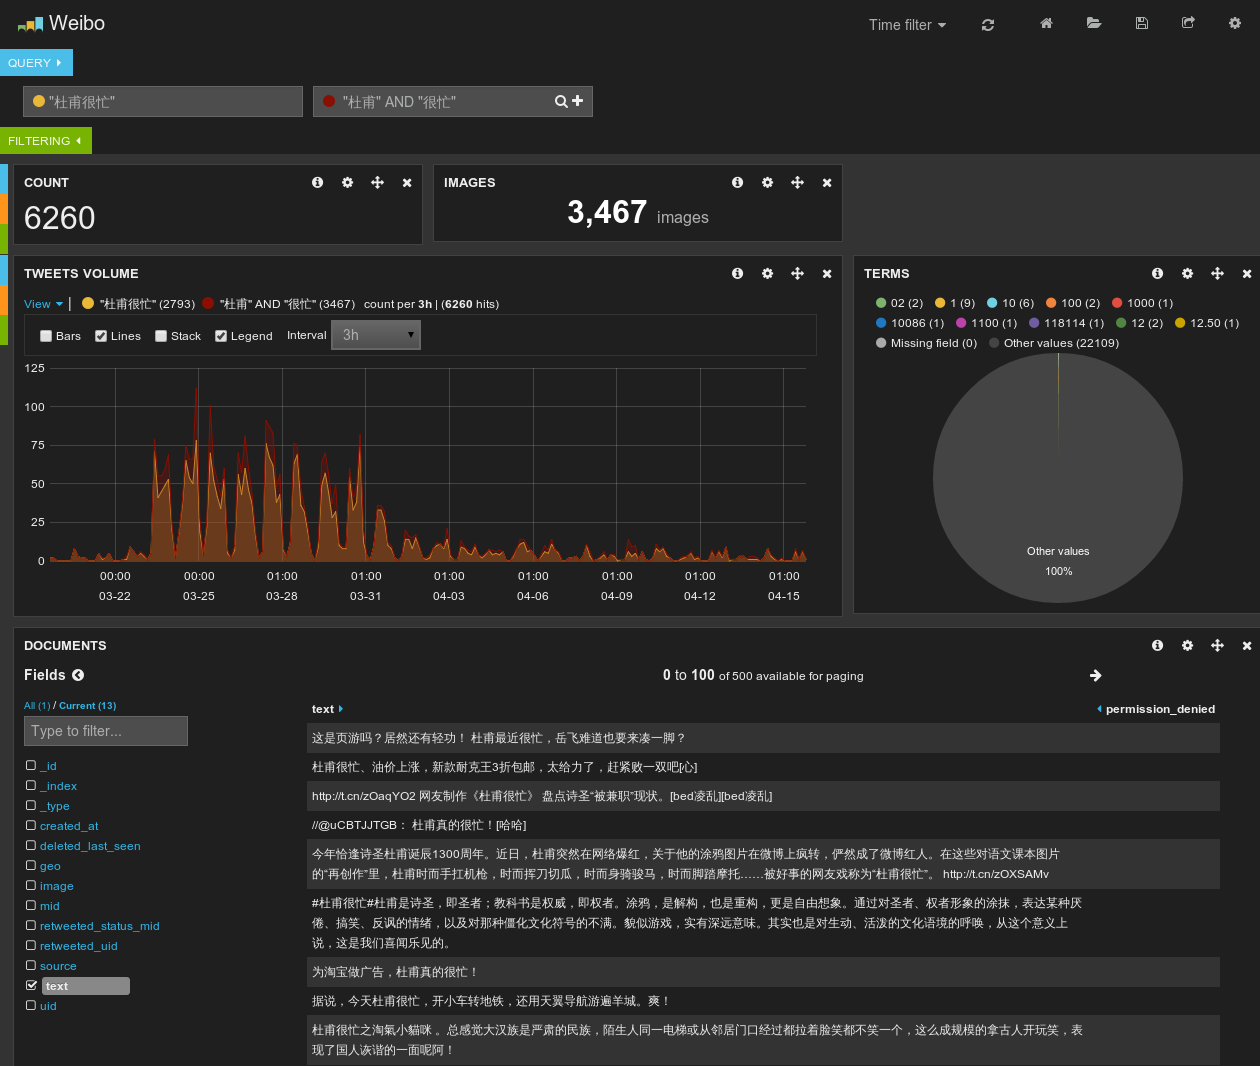
\includegraphics[width=6.0004in,height=5.078in]{figures/chap3/chapitre3-img20.png}
    \caption[Tableau de bords requêtes par mots-clés] { Ce tableau de bord permet de comparer la qualit\'e de diff\'erentes requ\^etes dans le corpus. Capture d'écran réalisée le 23 Mars 2014 à 16h18}
\end{figure}


Cette \'etape nous a \'egalement permis d{\textquoteright}identifier les
mots-cl\'es les plus appropri\'es pour d\'efinir chaque m\`eme. En
effet, la qualit\'e des archives pour chaque m\`eme d\'epend fortement
de la m\'ethode utilis\'ee pour collecter les donn\'ees. Ici, nous
utilisons la recherche plein texte pour collecter les donn\'ees et nous
devons ainsi nous assurer que notre requ\^ete est bien construite, afin
de minimiser le bruit dans chaque corpus (\'eviter les messages
contenant les m\^eme mots-cl\'es mais sans relations avec le m\`eme). 

Une fois assur\'e qu{\textquoteright}un m\`eme pouvait \^etre
correctement repr\'esent\'e dans un corpus de donn\'ees, nous obtenons
donc une liste r\'eduite de m\`emes \`a \'etudier pour chaque
cat\'egorie.

% \begin{figure}
    \centering
%     \centering
%     \begin{tabular}{c|c|c|c}

%         start & 
%         Name &  
%         type &  
%         keywords \\

%         February 3, 2012 & 
%         Campagne contre les touristes chinois à HK & 
%         Actualité, satire, commentaire social &
%         \zh{蝗蟲天下,蝗虫天下} \\

%         March 21, 2012 &
%         Détournement calligraphie : “Du Fu is very busy" &
%         Absurdiste, humour &
%         \zh{杜甫很忙,李白不服气了} \\

%         April 22, 2012 &
%         Chen Guancheng s'évade et se réfugie à l'ambassade des US &
%         Marketing politique, soutien, pétition &
%         \zh{陈光诚} \\

%         May 30, 2012 & 
%         Rumeur d'un coup d'état des proches de Boxilai (commentaires bloqués) &
%         Marketing politique, soutien, pétition & 
%         \zh{薄熙来,Zhou Yongkang} \\

%         July 13, 2012 &  
%         The Voice : lancement de l'émission TV &
%          Fan clubs, adoration & 
%         \zh{中国好声音, 吴莫愁} \\

%         July 15, 2012 &  
%         Gangnam Style : lancement du clip &  
%         Fan clubs, adoration  &  
%         \zh{鸟叔,江南STYLE} \\

%         August 26, 2012 &
%         Yang Dacai, l'officiel "souriant" et le scandale des montres &   
%         Actualité, satire, commentaire social &  
%         \zh{表叔,表哥,微笑局长,杨达才} \\

%         September 21, 2012 & 
%         Sortie du iPhone5   &
%         Publicité, marketing viral & 
%         \zh{iPhone, 苹果, Apple} \\

%         October 1, 2012 & 
%         Blague : "Yuan Fang, qu'est-ce que tu en penses?"  & 
%         Absurdiste, humour & 
%         \zh{远芳,你怎么看?,我觉得此事有蹊跷,神探狄仁杰} \\

%         October 1, 2012 &
%         Série TV : The Emperor's Harem & 
%         Publicité, marketing viral &
%         \zh{后宫,回家的诱惑,宫 (宫锁心玉)} \\

%         October 11, 2012  &
%         Mo Yan reçoit le Prix Nobel de littérature &
%         Fan clubs, adoration  &
%         \zh{莫言,管谟业,2012诺贝尔文学奖,诺贝尔} \\

%         October 25, 2012 &
%         Ai Weiwei sort son clip "Caonima style"&
%         Actualité, satire, commentaire social &
%         \zh{草泥马style, 艾虎子}\\

%         November 8, 2012 &
%         18ème Congrès du Parti Communiste &
%         Marketing politique, soutien, pétition &
%         \zh{中国共产党第十八次全国代表大会,中共十八大,18大,十八大}\\

%         November 20, 2012 &
%         La sex tape de Lei Zhengfu publiée par un journaliste &
%         Actualité, satire, commentaire social &
%         \zh{雷政富}\\

%         December 3, 2012  &
%         Qiegao : échauffourées autour d'un gâteau du Xinjiang &
%         Actualité, satire, commentaire social &
%         \zh{切糕}\\

%     \end{tabular}
%     \caption[Liste d{\textquoteright}\'ev\`enements web importants pendant l{\textquoteright}ann\'ee 2012] 
% \end{figure}

\subsection{Extraction des graphes et traitement des donn\'ees brutes}
Une fois cette requ\^ete clairement identifi\'ee nous proc\'edons pour
chaque m\`eme \`a l{\textquoteright}extraction d{\textquoteright}un jeu
de donn\'ees contenant l{\textquoteright}ensemble des messages
correspondant \`a la requ\^ete d\'efinie. Ce jeu de donn\'ees est
ensuite compl\'et\'e par l{\textquoteright}ensemble des messages
mentionn\'es mais ne contenant pas le mot cl\'e (commentaires,
r\'eponses, etc.) afin d{\textquoteright}obtenir un ensemble de
messages repr\'esentatifs pour chaque m\`eme.

Nous proc\'edons ensuite au traitement de chaque corpus selon une
s\'erie de proc\'edures d\'efinies comme suit :

\subsubsection{Graphe langagi\`ere (langagier ?)}

Le texte de chaque message est analys\'e de fa\c{c}on \`a ne conserver
que les mots les plus importants. Cela s{\textquoteright}effectue en
cinq \'etapes successives : 

i
\begin{enumerate}
\item La phrase est segment\'ee (analyse de la langue chinoise) pour
obtenir un ensemble de mots du m\`eme.
\item A chacun des mots est associ\'e l{\textquoteright}ensemble des
utilisateurs l{\textquoteright}ayant mentionn\'e.
\item Les mots les plus courants sont enlev\'es afin de r\'eduire le
bruit. La constitution de la liste des mots courants
\textit{(stopwords) }est une \'etape tr\`es importante. La liste que
nous utilisons a \'et\'e cr\'e\'ee \`a partir de diff\'erents corpus
lors d{\textquoteright}exp\'erimentations pr\'ec\'edentes et
augment\'ee de nouveaux mots au fur et \`a mesure.
\item La co-occurence d{\textquoteright}un mot dans une m\^eme phrase
d\'efinit une relation entre ces deux mots.
\item Parmi l{\textquoteright}ensemble de mots-cl\'es ainsi obtenu, nous
conservons les 500 mots les plus utilis\'es (dont les occurences sont
les plus nombreuses) 
\item Nous reconstituons le graphe des relations entre ces 500
mots-cl\'es d{\textquoteright}apr\`es la s\'erie de leur co-occurence :
chaque mot est un node, chaque co-occurence est un edge.
\item L{\textquoteright}ensemble constitue le graphe s\'emantique du
m\`eme, pond\'er\'e mais non dirig\'e.
\end{enumerate}
\textbf{3.4.2.2. Graphe conversationnel}

Pour chaque m\`eme, l{\textquoteright}ensemble des interactions
(mentions, citations et retweets) consituent le graphe conversationnel
o\`u un utilisateur est un node et une interaction est un edge. Le
graphe est dirig\'e car les interactions vont depuis un utilisateur \`a
un autre. 

Une fois l{\textquoteright}ensemble du graphe constitu\'e, nous
d\'eterminons sa modularit\'e et son coefficient moyen de clustering
afin de poss\'eder des informations sur sa structure. Nous calculons
\'egalement la centralit\'e interm\'ediaire (\textit{betweenness
centrality}) pour chaque utilisateur dans l{\textquoteright}ensemble du
graphe. Ensuite, nous identifions les diff\'erentes communaut\'es en
utilisant l{\textquoteright}algorithme dit de Louvain et son
impl\'ementation par Blondel \& al. \cite{Blondel2008}\footnote{
\url{http://perso.crans.org/aynaud/communities/index.html} consult\'e
le 22 Avril 2014 \`a 14:24} qui nous permet d{\textquoteright}attribuer
\`a chaque utilisateur un groupe unique. Enfin, nous r\'eduisons la
taille du graphe final en ne conservant que les utilisateurs ayant
effectu\'e au moins 2 \'echanges - en supprimant les \textit{edges} du
graphe ayant un poids inf\'erieur \`a 2.

Le graphe ainsi constitu\'e correspond aux donn\'ees conversationnelles
du m\`eme.

\subsubsection{Localisation des utilisateurs}

Pour chaque m\`eme, nous souhaitons \'egalement regrouper les
informations de localisation des utilisateurs mentionn\'es ou actifs
dans le m\`eme. Le jeu de donn\'ees \textit{Weiboscope }comprend les
localit\'es mentionn\'ees par les utilisateurs dans leurs profils. Le
nombre de ces localit\'es est restreinte par
l{\textquoteright}interface de Sina Weibo elle-m\^eme \`a :
l{\textquoteright}ensemble des provinces de Chine continentale, Hong
Kong, Macau, Taiwan, {\textquotedblleft}\`a
l{\textquoteright}\'etranger{\textquotedblright} et
{\textquotedblleft}autres{\textquotedblright}. Ainsi, pour chaque
utilisateur nous assignons l{\textquoteright}information g\'eographique
mentionn\'ee par l{\textquoteright}utilisateur dans son profil.

\subsection{Visualisation multi-graphes}
Une fois que l{\textquoteright}ensemble de ces donn\'ees a \'et\'e
extrait et trait\'e, nous pouvons consid\'erer diff\'erents aspects au
sein du m\`eme :

ii
\begin{itemize}
\item Graphe s\'emantique : mots-cl\'es et relations entre les mots
\item Graphe socio-s\'emantique : relations entre les mots et les
utilisateurs
\item Graphe conversationnel : relations et communaut\'es
d{\textquoteright}utilisateurs 
\item Graphe socio-g\'eographique : relations entre les utilisateurs et
les provinces / villes chinoises
\end{itemize}
Nous avons donc plusieurs niveaux de lecture interd\'ependants qui nous
permettent de consid\'erer diff\'erents aspects de chaque m\`eme.
N\'eanmoins, les informations de graphe sont peu claires et
difficilement exploitables sous forme de donn\'ees, \`a
l{\textquoteright}exception d{\textquoteright}une s\'erie de mesures
indicatives sur leurs structures. Afin d{\textquoteright}explorer ces
diff\'erentes relations, il nous faut pouvoir visualiser diff\'erentes
dimensions du m\`eme afin d{\textquoteright}observer les articulations
et ph\'enom\`enes possibles \'emergents de cette lecture. 

Pour r\'ealiser cette cartographie particuli\`ere, il
n{\textquoteright}existe pas d{\textquoteright}outils disponibles
permettant de mettre en relation diff\'erents types de r\'eseaux. Nous
avons donc choisi de d\'evelopper une solution technologique adapt\'ee
\`a nos besoins permettant de consid\'erer sous diff\'erents angles
l{\textquoteright}ensemble de ces graphes et de leurs relations. Les
diff\'erents choix conceptuels et technologiques pr\'esidant au design
de cet outil de visualisation sont d\'etaill\'es ci-apr\`es.

\subsubsection{Choix technologiques}

Les choix technologiques effectu\'es lors de toute cette recherche et
plus particuli\`erement pour cet outil de visualisation ont vocation
\`a faciliter l{\textquoteright}interop\'erabilit\'e et la publication
des r\'esultats (visualisation, code et donn\'ees) en ligne. Egalement,
l{\textquoteright}ensemble de l{\textquoteright}outil de visualisation
se fonde sur HTML5, CSS3 et Javascript qui sont des langages ouverts
issues d{\textquoteright}un travail collectif de
l{\textquoteright}ing\'enierie du Web permettant la r\'eutilisation
partielle ou totale des travaux produits par d{\textquoteright}autres
et contribuant ainsi \`a davantage
d{\textquoteright}interop\'erabilit\'e entre les diff\'erents design
scientifiques de recherche. La mise en forme des donn\'ees utilise la
librairie {\textquotedblleft}Data-Driven Documents{\textquotedblright}
(d3.js)\footnote{ D3js at \url{http://d3js.org/,} consult\'e le 24
Avril 2014 \`a 14:58}, les donn\'ees elles-m\^emes sont stock\'ees en
JSON pour les graphes et GeoJSON pour les donn\'ees cartographiques.

\subsubsection{Espace perceptif, plan projectif et choix
d{\textquoteright}un {\textquotedblleft}layout{\textquotedblright}}

Devant la disparit\'e des donn\'ees en pr\'esence, nous devons donc
construire un espace de repr\'esentation ou plut\^ot une interface de
repr\'esentation propice \`a l{\textquoteright}exploration et la
d\'ecouverte des ph\'enom\`enes dans les relations entre les
diff\'erents graphes. Dans la d\'efinition de cet espace perceptif se
joue la r\'econciliation d{\textquoteright}entit\'es dissemblables (des
utilisateurs, des lieux, des mots, leurs relations mutuelles). La
t\^ache consisterait ainsi \`a r\'econcilier dans le plan de
l{\textquoteright}espace graphique de la visualisation (ici celui de
l{\textquoteright}\'ecran) les diff\'erents espaces o\`u projeter ces
diff\'erents graphes. A l{\textquoteright}image du milieu num\'erique,
l{\textquoteright}existence m\^eme de ce plan r\'econciliant global,
local, r\'eel, symbolique et imaginaire pose question. A la simple
question : {\textquotedblleft}quelle doit \^etre sa
couleur?{\textquotedblright}, une logique commune de lisibilit\'e
r\'epondrait : {\textquotedblleft}blanc ou noir{\textquotedblright},
mais quelle peut en \^etre la justification logique dans
l{\textquoteright}espace de la visualisation? Et que penser du cot\'e
de l{\textquoteright}\'ecran? De quoi est-t-il le bord? D\`es lors que
se pose la question de structurer un espace de perception, nous voil\`a
devant plusieurs difficult\'es formelles majeures.
L{\textquoteright}exigence de rigueur scientifique et surtout
l{\textquoteright}imperm\'eabilit\'e des formats de publications
scientifiques actuelles rajoutent \`a la compexit\'e de cette
entreprise.

Afin de pouvoir consid\'erer les relations entres mots, communaut\'es et
territoires, nous devons dans l{\textquoteright}espace graphique
disponible, il est n\'ecessaire de r\'esoudre plusieurs probl\`emes :

ii
\begin{itemize}
\item Donner \`a voir chaque type d{\textquoteright}entit\'es de
fa\c{c}on reconnaissable (provinces chinoises, communaut\'es, mots)
\item Donner \`a voir les relations entre les diff\'erentes entit\'es
(graphe multiples)
\item Pallier l{\textquoteright}augmentation de la complexit\'e visuelle
et pr\'eserver une lisibilit\'e
\end{itemize}
Nous avons donc choisi de construire un espace sur plusieurs niveaux
hi\'erachis\'es.

\subsubsection{Graphes et interactions}

Le centre de la visualisation est occup\'e par les utilisateurs,
refl\'etant \`a la fois l{\textquoteright}int\'er\^et central de cette
\'etude pour l{\textquoteright}\'etude des processus
d{\textquoteright}individuation et le r\^ole charni\`ere des
utilisateurs dans la structuration des donn\'ees. Plus exactement, nous
avons choisi de regrouper les utilisateurs par communaut\'es afin de
consid\'erer les liens qui les unissaient entre elles et la structure
g\'en\'erale de la discussion plut\^ot que de
s{\textquoteright}int\'eresser aux individus. Les individus sont
symbolis\'es par des points au sein des communaut\'es dont la couleur
indique leur centralit\'e dans le r\'eseau global. 

Notre premi\`ere id\'ee a \'et\'e de repr\'esenter
l{\textquoteright}ensemble des utilisateurs sur une carte pour
comprendre comment s{\textquoteright}agencaient spatialement chacune
des discussions. La premi\`ere \'etape a donc \'et\'e de reconstituer
une carte de la Chine comprenant Taiwan, Hong Kong et Macau. Chacun de
ces territoires poss\`edent une influence m\'ediatique certaine en
Chine et m\'eritent \`a ce titre d{\textquoteright}\^etre
repr\'esent\'e. N\'eanmoins, le statut politique particulier de chacun
de ces territoires nous a oblig\'e \`a reconstituer une carte o\`u ils
figuraient tous. Nous avons choisi d{\textquoteright}aggrandir
l{\textquoteright}\'echelle de Hong Kong et Macau afin
qu{\textquoteright}il soit visible sur la carte. Egalement, nous avons
choisi de ne pas restituer les donn\'ees concernant les utilisateurs
ayant choisi {\textquotedblleft}autres{\textquotedblright} ou
{\textquotedblleft}reste du monde{\textquotedblright} comme leurs lieux
de r\'esidence.

Si la carte se pr\^ete assez bien \`a la visualisation de quantit\'e,
les visualisations de graphe deviennent facilement confuses. Ainsi,
nous avons choisi d{\textquoteright}ajouter une option de visualisation
des provinces sous la forme d{\textquoteright}une liste, au moins toute
aussi parlante. Cela nous permet en plus d{\textquoteright}organiser
cette liste selon diff\'erents crit\`eres afin
d{\textquoteright}\'etudier plusieurs aspects qui peuvent \^etre
int\'eressants.

Le graphe de mots rev\^et ici la forme la plus simple. Les relations
entre les mots sont mat\'erialis\'ees par un graphe utilisant un
algorihme force-based pour disposer les mots entre eux, recr\'eant
ainsi des groupes de mots int\'eressants d{\textquoteright}apr\`es leur
proximit\'e dans les phrases lors des discussions. Un positionnement
des mots selon leur importance (nombre de citations) est \'egalement
disponible \`a loisir.

Afin d{\textquoteright}explorer les diff\'erentes dimensions du graphes,
nous avons \'egalement ajout\'e des interactions qui permettent de
focaliser sur des zones ou des caract\'eristiques pr\'ecises des
graphes. \cite{Bostock2011}

\begin{figure}
    \centering
    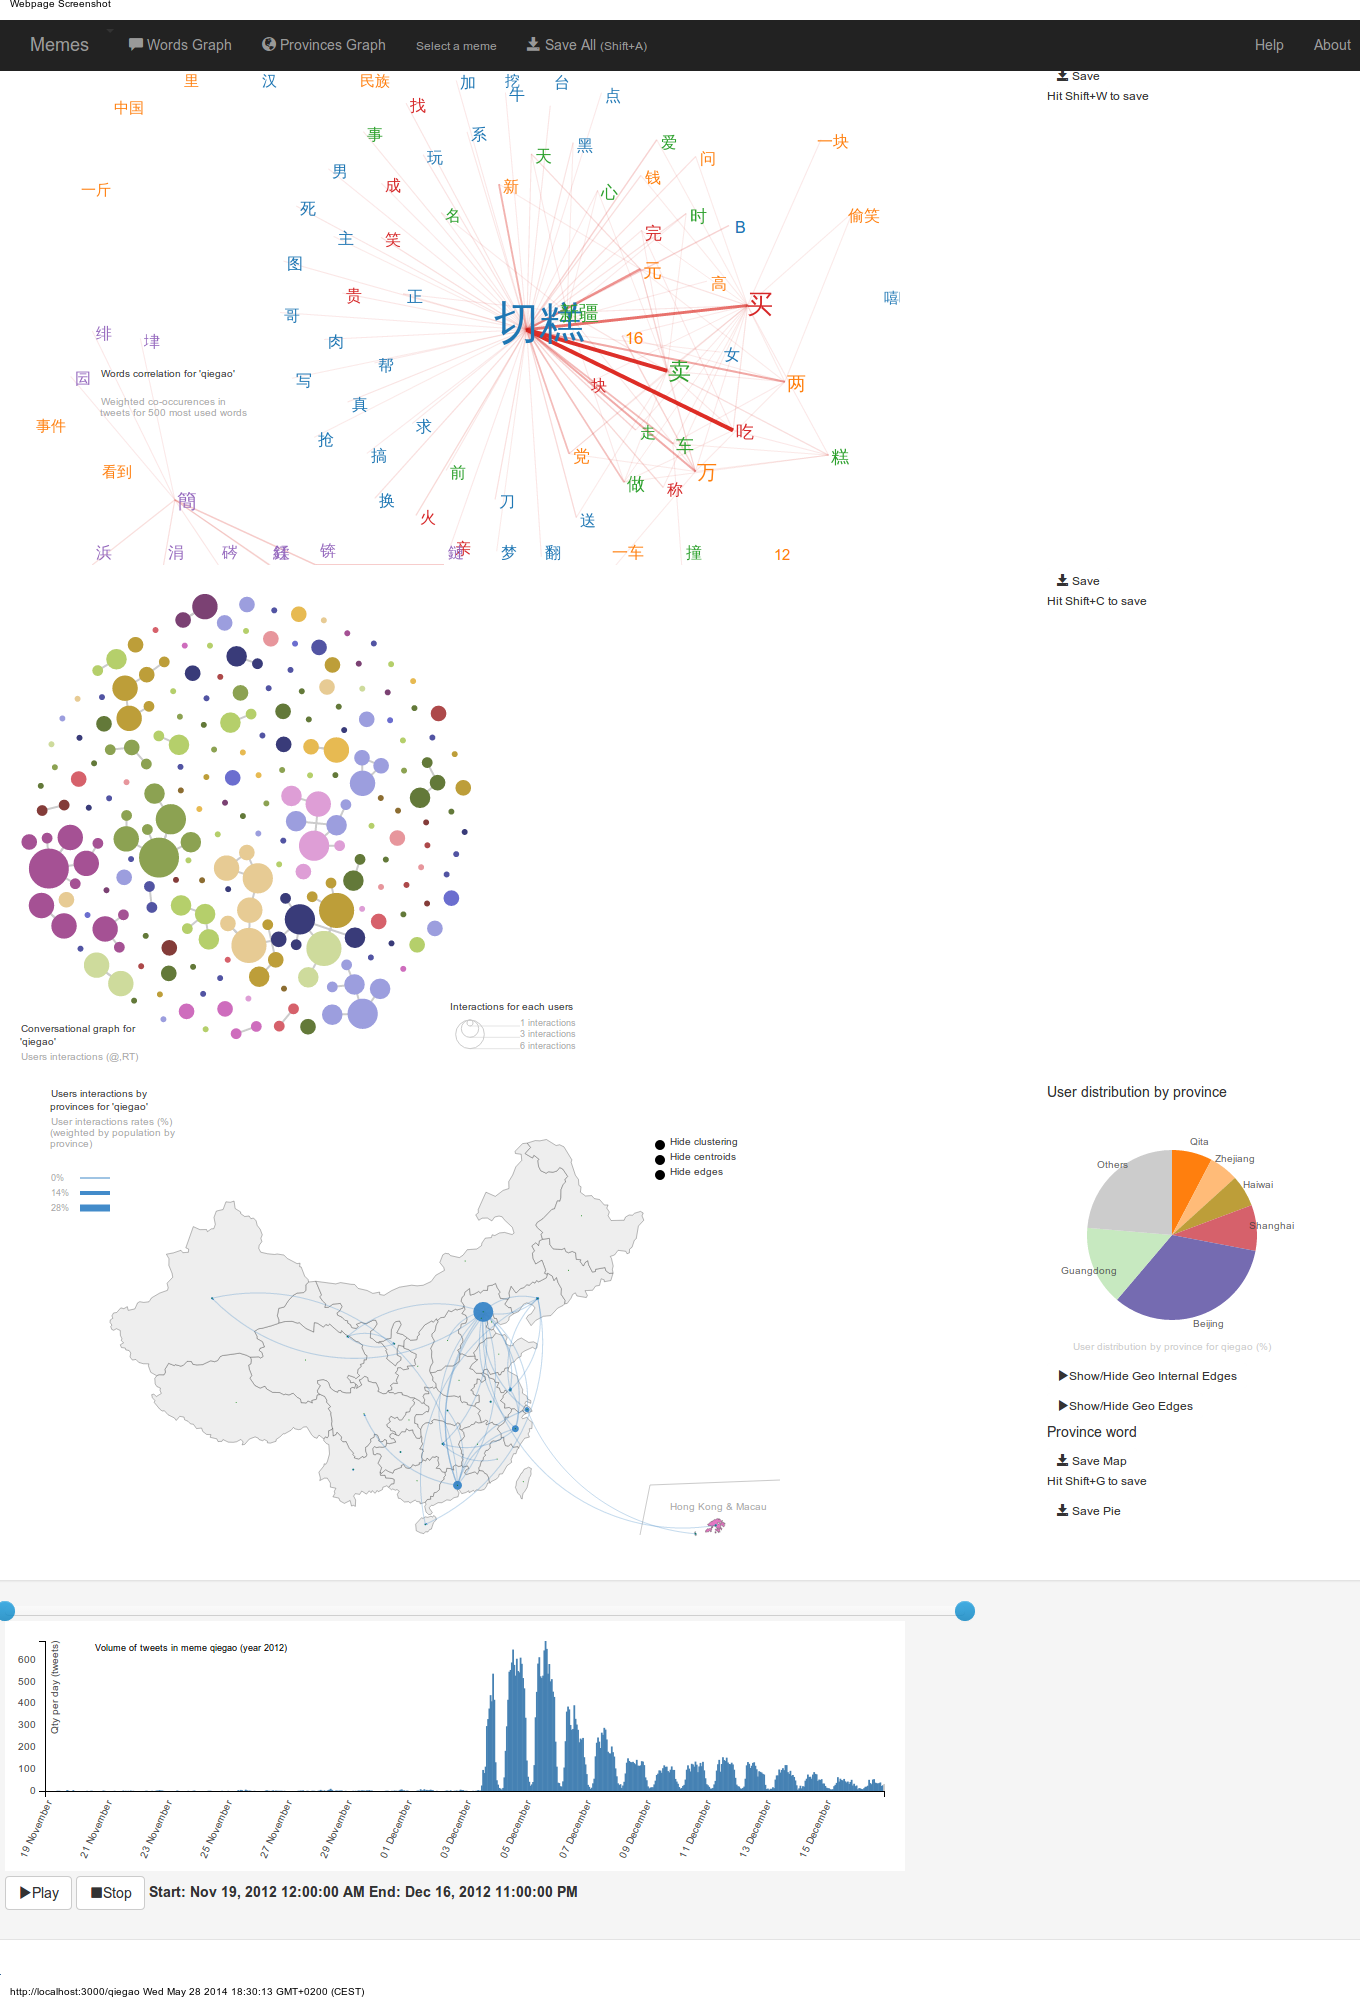
\includegraphics[width=6.7213in,height=8.3894in]{figures/chap3/chapitre3-img21.png}
    \caption{Interface d'exploration et de visualisation des données}
\end{figure}